\documentclass[12pt,a4paper]{article}
\usepackage[margin=1in]{geometry}

\usepackage[utf8]{inputenc}
\usepackage[T1]{fontenc}
\usepackage{url}
\usepackage{booktabs}
\usepackage{amsfonts}
\usepackage{nicefrac}
\usepackage{microtype}
\usepackage{lipsum}
\usepackage{float}
\usepackage{caption}
\captionsetup[figure]{font=small,labelfont=small}
\captionsetup[table]{font=small,labelfont=small}
\usepackage{amsmath}
\usepackage{lscape}
\usepackage{setspace}
\usepackage{natbib}
\renewcommand{\rmdefault}{ptm}
\usepackage{eurosym}
\usepackage[pdftex]{graphicx}
\usepackage{tikz}
\usepackage{authblk}
\usepackage{dcolumn}
\usepackage{multirow}
\usepackage{hyperref}
\hypersetup{colorlinks=true,linkcolor=blue,urlcolor=blue,anchorcolor=blue,citecolor=blue}
\usepackage{bibunits}
\defaultbibliographystyle{apalike}
\newcommand{\sym}[1]{{#1}}
\usepackage{afterpage}
\usepackage{comment}

\providecommand{\keywords}[1]
{
  \small	
  \textbf{\textit{Keywords---}} #1
}

\title{The Economics and Econometrics of \\ Gene--Environment Interplay}

\author{
 Pietro Biroli\thanks{University of Bologna. E-mail: \href{mailto:Pietro.Biroli@econ.uzh.ch}{pietro.biroli@unibo.it}.}, 
 \hspace{0.5cm} 
 Titus Galama\thanks{University of Southern California and VU University Amsterdam. E-mail: \href{mailto:galama@usc.edu}{galama@usc.edu}.}, 
 \hspace{.5cm} 
 Stephanie von Hinke\thanks{University of Bristol; Institute for Fiscal Studies. E-mail: \href{mailto:S.vonHinke@bristol.ac.uk}{s.vonhinke@bristol.ac.uk}.}, 
 \\ \hspace{.5cm} 
 Hans van Kippersluis\thanks{Corresponding author: Erasmus University Rotterdam. E-mail:  \href{mailto:hvankippersluis@ese.eur.nl}{hvankippersluis@ese.eur.nl}.}, 
 \hspace{.5cm} 
 Cornelius A. Rietveld\thanks{Erasmus University Rotterdam. E-mail:  \href{mailto:nrietveld@ese.eur.nl}{nrietveld@ese.eur.nl}.}, 
 \hspace{.5cm} 
 Kevin Thom\thanks{University of Wisconsin. E-mail: \href{mailto:thomk@uwm.edu}{thomk@uwm.edu}.}
} %end author

\begin{document}

\begin{bibunit}

\maketitle

\begin{abstract}
\noindent We discuss how to estimate the interplay between genes (nature) and environments (nurture), with an empirical illustration of the moderating effect of school-starting age on one's genetic predisposition towards educational attainment. We argue that gene--environment ($G \times E$) studies can be instrumental for (i) assessing treatment effect heterogeneity, (ii) testing theoretical predictions, and (iii) uncovering mechanisms, thereby improving understanding of how (policy) interventions affect population subgroups. Empirically, we find that being old-for-grade and having a higher genetic propensity for education benefits children on assessment tests as they progress through school. In this setting, families appear to increase genetic inequalities while schools seem to reduce them.
\end{abstract}

\small
\noindent \textbf{\textit{Keywords}:} ALSPAC; \and Gene-environment interplay; \and Genoeconomics; \and Polygenic indices; \and School entry policies; \and Social science genetics \\
\textbf{\textit{JEL Classifications}:} D1, D3, I1, I2, J1
\normalsize

\bigskip 

\clearpage
\onehalfspacing



%------------------------------------------------------------------------------------------------------%
\section{Introduction}
\label{sec:intro}

The debate over the relative importance of nature versus nurture in the development of human traits is amongst the oldest in the social sciences. Decades of twin studies have demonstrated that genetic factors account for approximately 25-75\% of the between-individual variation in a wide range of behaviors, traits, and outcomes \citep{Polderman2015}.  This finding is summarized in the \textit{first law of behavioral genetics}: ``all human behavioral traits are heritable'' \citep{Turkheimer2000}. Of course, environmental factors are similarly important.  Moreover, genes and environments do not operate in isolation.  Gene-by-environment ($G \times E$) interaction occurs when environmental factors influence the relationship between the genotype and the outcome of interest, or vice versa.\footnote{Gene--environment interplay differs from the study of epigenetics, which focuses on the role of gene \textit{expression}. Whereas individuals' genotype is fixed at conception, their gene expression may change over the life course due to environmental influences. As such, epigenetic processes can provide one explanation for the existence of gene--environment interplay, but they are not the only possible mechanism. See \hyperref[appsec:epi]{Appendix~\ref*{appsec:epi}} for more details.}    Most outcomes arise from a web of both genetic and environmental influences that may interact in complex ways \citep{Hunter2005, Heckman2007}.

Rapid reductions in the cost of collecting and processing genetic material have expanded the availability of genetic data, making it feasible to study complex $G \times E$ interplay in econometric analyses.  Single-nucleotide polymorphisms or SNPs (pronounced ``snips'') represent the most common type of genetic variation, and occur when individuals differ in the molecules they possess at specific positions on the genome.  With the ability to measure SNP-level variation, researchers can study the influence of a single SNP, or the combined influence of millions of SNPs aggregated into a polygenic index (PGI).\footnote{Different terms are used to refer to the genetic component, including genotype, genetic makeup, genetic propensity, genetic endowments, genetic variants, polygenic scores (PGS), and PGI. The Glossary in \hyperref[appsec:glossary]{Appendix~\ref*{appsec:glossary}} provides definitions of the most important genetic terminology used in the paper.}  
PGIs have substantially greater predictive power than do single SNPs, and are now available in many rich (longitudinal) datasets. Since anyone can now explore the role of $G \times E$ in shaping individual outcomes, even without much knowledge of genetics, economists need to be aware of the complexities of genetic data and the interpretation of $G \times E$ results.  We aim to provide this essential guidance here.

We build on previous surveys of the use of genetic data in economic analyses\footnote{Examples include \citet{Benjamin2011}, \citet{Beauchamp2011}, and \citet{benjamin2024social}, and more specifically the surveys on $G \times E$ interplay, as in \citet{Fletcher2013} and \citet{Schmitz2017}. See \cite{Rutter2006}, \citet{Plomin2014}, \citet{Mills2020book} and \citet{domingue2020interactions} for related work in other disciplines.}, and focus on the economics and econometrics of $G \times E$ interplay. Our contribution is twofold. In the first part of the paper we introduce key concepts, discuss recent developments in the field, and highlight the intricacies of understanding and interpreting $G \times E$ estimates. In the second part we offer practical guidance on how to use genetic data to explore nature--nurture interplay. We do this by testing for the presence of $G \times E$ interactions in the context of school entry policies in the United Kingdom. Specifically, we examine interactions between the age of school entry and a PGI for educational attainment (EA) in shaping performance on standardized tests throughout childhood, from ages 4 to 16. 

There is a long-standing debate \citep{heath1985education} on whether educational institutions moderate inequalities induced by the ``genetic lottery'' \citep{harden2021genetic}. 
Policies related to entry into the formal schooling system -- including the age of school entry -- are of particular interest since they determine the moment at which the bulk of skill development is transferred from parents to schools. 
With current, state-of-the-art EA PGIs explaining 12-16\% of the variation in educational attainment, on par with some of the strongest environmental determinants such as parental education and income \citep{lee2018gene, Okbay2022}, molecular genetic data can now be used to shed light on its role in shaping inequalities. 

In this paper, we study whether and how school-starting age moderates the relationship between genotype and academic achievement, and quantify the magnitude of such $G \times E$ effects. In the United Kingdom, strict birth-date cutoffs dictate that individuals born just before September 1 start formal schooling at age four (making them relatively young in their class), while those born on September 1 or just after start around age five (making them relatively old in their class).  This quasi-randomly assigned treatment is multifaceted, as the children born just after September 1 (i) enter school and take tests at an older age, (ii) are relatively older than their classmates, and (iii) receive an extra year of exposure to their parental rearing environments before starting formal schooling.  The existing literature -- discussed more extensively below -- has found that children who are older when they start schooling (and therefore also older relative to their peers) perform substantially better on grade-level tests.  

We estimate the treatment effect -- i.e., being old-for-grade -- on a series of five standardized tests.  The first test is taken upon entering primary school, i.e., before any exposure to formal schooling.  For this first test, we find a strong positive interaction between the genetic propensity for educational attainment (as measured by the EA PGI) and being old-for-grade. That is, old-for-grade children perform better on the entry assessment test, and high EA PGI children gain more, on average, from entering school later. Since these tests are taken before children enter school, the treatment reflects biological maturation and having spent more time at home (e.g., more parental investments). Interestingly, for standardized tests taken several years after the start of formal schooling, we generally find a pattern of negative interactions between assignment to old-for-grade and the EA PGI.  That is, children with lower EA PGI values gain more from being old-for-grade in the formal schooling system. In addition to reflecting biological maturation and more time at home, the treatment now also includes effects that operate through the school environment, suggesting that formal schooling reduces genetic inequality for EA. In \hyperref[sec:econModel]{Section~\ref*{sec:econModel}}, we discuss how a simple economic model can help with the interpretation of these opposing $G \times E$ estimates.

The study of $G \times E$ interplay may advance basic science by improving our understanding of the role of nature and nurture in shaping human capabilities. Beyond this, we contend that studying $G \times E$ interplay is of general interest, even for those with no inherent interest in the biological origins of economic outcomes, for at least three reasons:

(1) \textit{Treatment effect heterogeneity and inequality}:  Researchers and policy-makers are often interested in characterizing the distribution of treatment effects associated with a particular intervention or policy change.  Their impact depends on which individuals are most affected, and how they respond.  $G \times E$ studies can reveal whether and how individuals with different genetic endowments are differentially affected, extending our ability to describe treatment effect heterogeneity beyond standard observables. A review of recent papers in this literature, with a focus on educational attainment, suggests that $G \times E$ interactions are quantitatively important and around 1.5 to 3 times smaller than the main effects (see  \hyperref[sec:litreview]{Appendix~\ref*{sec:litreview}}). In our empirical analysis we find that old-for-grade children score 0.38 standard deviations higher on the standardized test taken at age 10-11, and this effect is 25\% higher for children with a PGI one standard deviation below the mean. 

Knowing whether a policy moderates differences arising from genes is of interest because people exhibit very different moral intuitions for inequalities arising from genetics or from early life socioeconomic conditions \citep[e.g.,][]{sandel2020tyranny,harden2021genetic}.   Some consider genetic gradients a signal of meritocracy \citep[e.g.,][]{Rimfeld2018}, whereas others view genetic differences as yet another layer of inequality of opportunity since genes -- like rearing environments -- are unchosen and unearned \citep[e.g.,][]{harden2021genetic, kweon2020genetic}. Understanding treatment effect heterogeneity arising from genes also holds a special significance for studying intergenerational mobility:  since genes are inherited, policies that benefit one generation may be propagated to the next and thereby affect long-run inequalities.

Results from $G\times{}E$ studies may also enable the targeting of scarce resources, or the development of personalized interventions.  In medicine, genetic data are already widely used for diagnostic purposes and for the tailoring of treatments.  $G \times E$ effects for complex economic outcomes like educational attainment raise the possibility of similar applications in skill development.  In the short run, it seems unlikely that school systems or other institutions would incur the substantial costs of creating personalized experiences informed by genetics. It is also debatable whether the use of genetic data will ever be informative and beneficial enough to justify its institutional use given the large ethical and privacy concerns \citep{meyer2023wrestling}. However, our empirical application highlights that $G \times E$ research might be more immediately useful at the level of household decision-making. Well-identified $G\times{}E$ studies are a prerequisite for assessing the viability of such applications. Even here, enthusiasm over such applications may be premature since the current predictive power of PGIs may be too low for useful \textit{individual}-level recommendations \citep{morris2020can,Turley2021embryo}. Still, depending on preferences and constraints, households on the margin could conceivably use genetic information as one input among many when deciding the best environment for their child. For example, our empirical results suggest that genetic information may help parents on the margin determine an appropriate age-at-entry into formal schooling within educational systems that allow such choice.    

(2) \textit{Testing theoretical predictions}:  Economic theory predicts that idiosyncratic characteristics like preferences, health endowments, and abilities shape individual choices and generate differences in how individuals respond to a common environmental change.  For example, models of skill formation often assume that parents actively respond to the endowments of their children \citep[e.g.,][]{becker1976child,behrman1997intrahousehold,CURRIE20111315}, and that abilities and endowments are productive complements with parental investments \citep[e.g.,][]{ben1967production,becker1986human,cunha2007technology}. Since primitive variables, such as endowments and abilities, are typically hard to measure, testing such predictions can be challenging. Observable genetic variation -- especially random variation within families --  offers a new and powerful way to measure such characteristics, and test theoretical predictions.  For example, \citet{breinholt2020child}, \citet{fletcher2020production}, \citet{Sanz-de-galdeano2022}, and \citet{houmark2020nurture} provide evidence that parental investments indeed respond to children's genotypes.   The presence (or absence) of $G \times E$ interactions can similarly test assumptions or theoretical predictions. For example, \citet{Muslimova2020b} find that children with higher EA PGI values relative to their siblings gain more from being the firstborn.  Since parental investments are a dominant channel driving birth order effects, these results are consistent with complementarity between genetic endowments and parental inputs in the formation of human capital. 

In our application, $G \times E$ results for age-at-entry have implications for the role of formal schooling and patterns of substitutability in the human capital production function.  Although high PGI students benefit the most from being older in terms of entry skills \textit{prior to the start of formal schooling}, low PGI students benefit the most in \textit{in-school} standardized testing. This combination of results suggests that being old-for-grade during the formal schooling years brings about a series of environments or investments that together act as technical substitutes for genetic endowments. These results place limits on how strongly past skills, genetic endowments, and being old-for-grade complement one another in the context of the formal schooling system.  

(3) \textit{Uncovering mechanisms}: Evidence on $G \times E$ interplay can also provide clues about the economic or behavioral mechanisms through which genetic factors operate. For example, \citet{barth2020genetic} find that access to defined benefit pension plans substantially moderate the relationship between the EA PGI and household wealth. This suggests that genetic endowments related to schooling influence household wealth not only through earnings and consumption-savings choices, but also through financial decision-making and portfolio choice. Researchers developing and estimating quantitative life-cycle models of these outcomes have to choose how to incorporate heterogeneity (e.g., which primitive parameters to make random, and what kinds of covariance structures to allow). Since genetic factors may constitute a substantial portion of  ``unobserved heterogeneity'', evidence on the mechanisms through which they operate may help guide modeling choices \citep{Benjamin2012}.  For example, the results from \citet{barth2020genetic} suggest that in life-cycle models of education and inequality, it may be important to allow sources of heterogeneity that shift education choices to be correlated with heterogeneity in primitive parameters relative to financial-decision making or rates of return on invested wealth. 
   
Finally, just as the empirical analysis of $G \times E$ can provide novel insights for economists, there is great potential to using the toolbox of economics to better design $G \times E$ studies and thus advance the field of genetics in general and social-science genetics in particular. Since $G \times E$ interplay often stems from endogenous behavioral adjustments, economic theory can help clarify why and when such interplay might occur and what it implies for policy. Empirically, both genetic endowments and environmental factors are typically endogenous in the study of a particular outcome. Ongoing advances in methods and data are creating opportunities for the causal inference of genetic factors. Economists have substantial experience with exploiting exogenous variation in environmental exposures and have developed a large toolbox to deal with endogeneity. Given the importance of establishing which causal environmental exposures moderate what genetic predispositions, economists are well-positioned to improve our understanding of the complex interplay between nature and nurture in shaping life outcomes. 

This paper is organized as follows. \hyperref[sec:G]{Section~\ref*{sec:G}} discusses the measurement of $G$, distinctions between environments that act as moderators or mediators of genetic effects, the interpretation of genetic effects, and how the natural experiment of genetic inheritance can be exploited to analyze causal genetic effects. 
In \hyperref[sec:specification]{Section~\ref*{sec:specification}}, we discuss the intricacies of interpreting an empirical $G \times E$ model, providing a systematic categorization of $G \times E$ analyses and a discussion of the direction and nature of the bias in $G$, $E$ and $G \times E$ for each case relative to the ideal (unbiased) case, in which both $G$ and $E$ are exogenous. 
Readers familiar with the (social science) genetics literature may wish to skip directly to \hyperref[sec:application]{Section~\ref*{sec:application}}, where we uncover a novel $G \times E$ interaction between being old-for-grade in school ($E$; exogenous due to sharp cut-offs in month of birth determining eligibility for school entry) and the genetic propensity for educational attainment ($G$; exogenous since the child's genotype is random conditional on the parental genotypes) on test scores at different ages throughout childhood. \hyperref[sec:discussion]{Section~\ref*{sec:discussion}} concludes by providing a brief discussion of our results. 

\section{Measuring and interpreting \textit{G}} 
\label{sec:G}
The following discussion assumes a minimum level of understanding of genetic concepts, with the Glossary in \hyperref[appsec:glossary]{Appendix~\ref*{appsec:glossary}} providing definitions of the genetic terminology used in the paper. We suggest that those new to genetics start with \hyperref[appsec:genes]{Appendix~\ref*{appsec:genes}} for a short primer.

More than 15 years of Genome-wide Association Studies (GWAS) show that virtually all outcomes that social science researchers are interested in are highly ``polygenic'' \citep{visscher2008heritability,Loos2020,Abdellaoui2023}. That is, there is no ``gene for'' a certain outcome, but individuals rather fall somewhere on a scale of the genetic predisposition to a certain outcome that reflects the aggregation of numerous small contributions of millions of genetic variants (Single Nucleotide Polymorphisms; SNPs). Most studies therefore tend to use PGIs \citep{Becker2021} instead of individual SNPs, where a PGI is a weighted sum of individual SNPs. 

While a PGI constitutes the best linear genetic predictor of an outcome \citep{Mills2020book,Becker2021}, it is important to emphasize that this holds within the environmental and demographic context of the discovery sample \citep{Mills2020book, domingue2020interactions}. Most existing PGIs are derived from discovery samples based on European-ancestry populations, with limited `portability' to populations with different ancestries \citep{benjamin2024social}. Thus, the association between a PGI and an outcome cannot be interpreted as an immutable biological relationship \citep[e.g.,][]{mostafavi2020variable,kweon2020genetic}: the effects depend on the context, i.e., on the environment. For example, even though alcohol metabolism and dependence are partially determined by genetic factors, in an environment where alcohol consumption is illegal or low because of cultural reasons  \citep{cho2015alcohol}, the genetic effects would be (close to) zero.

Environmental factors may influence the relationship between the PGI and the outcome of interest through at least three channels: as \textit{moderators, confounders}, and \textit{mediators}. As a \textit{moderator}, the environment could change the strength of the relationship between a PGI and the outcome. This is precisely the topic of this paper, where environmental moderation would be reflected by the $G \times E$ interaction term.

To understand the environment as a \textit{confounder} and \textit{mediator} of the PGI effect, we consider educational attainment as the outcome variable. \autoref{fig:diagram} shows a schematic of the relationships between the parental genotypes ($G_{father}$ and $G_{mother}$), the environment ($E_{child}$), the child's genotype ($G_{child}$) and the child's outcome ($Y_{child}$). The top part of the diagram shows how the genotypes of mothers and fathers may be correlated through assortative mating.\footnote{Assortative mating based on educational attainment and correlated characteristics has been shown to induce a non-negligible correlation in genotypes across mothers and fathers in the order of 0.10-0.20 \citep[e.g.,][]{robinson2017genetic,morris2020population,torvik2022modeling,collado2023estimating}.} The arrow from $G_{father}$ and $G_{mother}$ to $G_{child}$ (genetic recombination) reflects the notion that a child inherits her genotype from her parents through recombination of the parental genotypes. The child's genotype in turn has a direct effect on the outcome (arrow from $G_{child}$ to $Y_{child}$, ``direct effect''), while the parental genotypes may be associated with the environment (arrow from $G_{mother}$ and $G_{father}$ to $E_{child}$). That is, parents with genotypes conducive to education may provide an environment more beneficial to their child's learning \citep[so-called genetic nurture;][]{Bates2018,Kong2018,Wertz2018}, and/or genotypes of parents may simply be correlated with environmental advantages that originate from older ancestries \citep[so-called dynastic effects,][]{nivard2024more}. This environment in turn may raise the child's educational achievement (arrow from $E_{child}$ to $Y_{child}$). Here, the child's environment acts as a \textit{confounder} because $E_{child}$ not only influences the outcome $Y_{child}$ but is also correlated with the child's genotype $G_{child}$ through the parental genotypes. Genetic nurture and dynastic effects are examples of a so-called ``passive gene--environment correlation'' ($rGE$) (double thin arrow between $G_{child}$ and $E_{child}$), which occurs when individuals' genotypes relate to their environment, but that environment is not a consequence of the child's genotype $G_{child}$.\footnote{Passive $rGE$ also occurs when siblings' genotypes partially shape the environment that individuals are exposed to \citep[e.g.,][]{cawley2019testing}. Since siblings share, on average, 50\% of their DNA, this introduces a correlation between sibling genotypes and sibling environments. However, conditional on parental genotypes, the child's genotype is as good as random, fully eliminating any confounding due to passive $rGE$ (as we discuss later).} 

\begin{figure}[ht]
    \centering
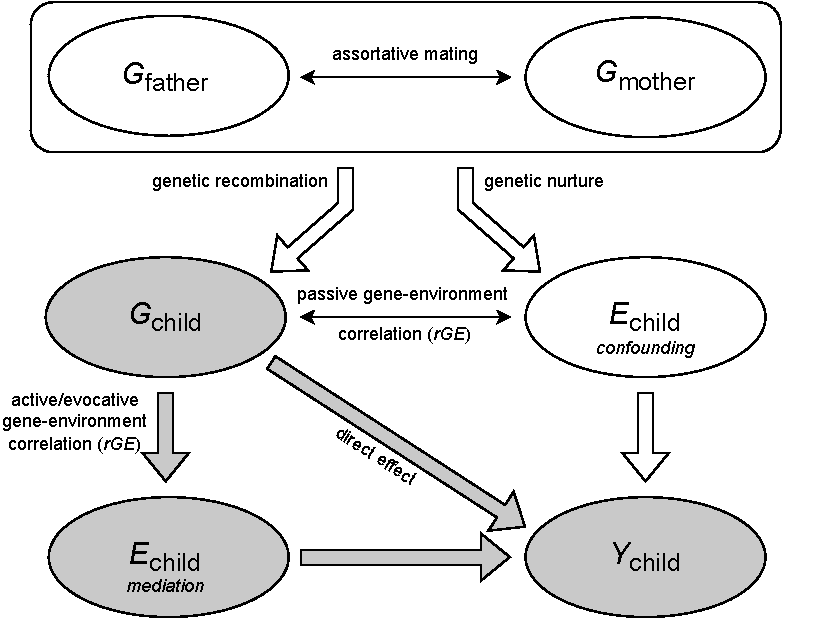
\includegraphics[width=10cm]{include/GxEtest_alt3.drawio.pdf}

    \caption{The relationships between parental genes ($G_{father}$ and $G_{mother}$), the child's genes ($G_{child}$), environmental factors ($E_{child}$), and the outcome ($Y_{child}$). The grey area represents the ``causal'' region of the diagram (explained further in the text).
    }
    \label{fig:diagram}
\end{figure}

In general, gene--environment correlation ($rGE$) describes the phenomenon of certain environments being more prevalent among carriers of certain genotypes \citep{Plomin1977,Fletcher2013}. In addition to \textit{passive} $rGE$, there are two other types of $rGE$: active and evocative $rGE$ \citep{Plomin1977}. \textit{Active} gene--environment correlation occurs when individuals with certain genotypes self-select into certain environments $E_{child}$  (``mediation''). For example, someone with a high genetic predisposition for education may find it easier to apply for and be accepted into a selective, high-quality university. \textit{Evocative} gene--environment correlation occurs when someone's genetic predisposition $G_{child}$ invokes a certain environmental response; $E_{child}$ (``mediation''). For example, a child with a high genetic predisposition for calmness may be treated differently by her parents and teachers, creating an environment that may be more conducive to learning. Hence, both active and evocative $rGE$ imply that the environment $E_{child}$ is a \textit{consequence} of the child's genotype $G_{child}$. These environments, in turn, may influence the child's educational attainment $Y_{child}$. Hence, through active and evocative $rGE$, the environment may act as a \textit{mediator}, a variable that is influenced by the child's genotype $G_{child}$ and that in turn influences the outcome $Y_{child}$.

Genotypes have the useful property of being fixed at conception. Thus, the outcome cannot affect the genotype (i.e., there is no reverse causality). We adopt the view that the causal effect of genotype can be thought of as a \textit{variant substitution} effect \citep{lee2013causal,morris2020population}. That is, the causal effect of a genetic variant is the counterfactual change in an individual's outcome that would occur had that genetic variant been different at conception, with all else held constant.\footnote{Other definitions, e.g. \citet{young2022mendelian}, also include indirect genetic effects stemming from passive $rGE$ as part of the causal effect of $G$. From a dynastic point of view, these definitions are similar---hypothetically, a change in one's genotype at conception will have implications for individuals and their offspring (i.e., may lead to passive $rGE$ for the next generation). We here take an individual's genotype as the relevant unit of analysis and therefore treat passive $rGE$ arising from relatives' genotypes as a source of bias rather than a causal effect.} 
In the diagram, the mechanisms through which the child's genotype $G_{child}$ operate can be through direct pathways (e.g., gene expression) but can also be environmentally driven (e.g., through active or evocative $rGE$). Both direct and indirect genetic pathways fall within the causal part of the diagram (shown in gray). 

The existence of (passive) $rGE$ implies that the offspring's genotype $G_{child}$ and outcome $Y_{child}$ are simultaneously influenced by the parental genotypes. This implies that the offspring genotype $G_{child}$ is endogenous. As we discuss in \hyperref[subsec:ideal]{Section~\ref*{subsec:ideal}}, controlling for the parental genotype can fully address confounding due to passive $rGE$, allowing for causal inference. This is because, conditional on the parental genotypes, the child's genotype is as good as random (``Mendel's Law''), breaking the link between child genotype $G_{child}$ and the confounding child environment $E_{child}$.\footnote{This property is also exploited in so-called Mendelian randomization studies that use genotypes as instrumental variables for endogenous environmental exposures \citep{VonHinke2016}. Mendel's law also allows for calculating the expected relatedness among offspring given the relatedness of the parents. Deviations from expected relatedness (``relatedness disequiblibrium'') are due to random segregation and can therefore be used to estimate a trait's heritability free from environmental bias \citep{young2018relatedness}.
} Controlling for parental genotypes can also solve biases arising from assortative mating, which typically inflates the association between $G_{child}$ and the outcome $Y_{child}$ \citep{young2023estimation}.\footnote{Assortative mating on educational attainment induces a correlation across SNPs that influence the genetic propensity to educational attainment in future generations. It can be thought of as a form of population stratification (see also \hyperref[appsec:gwas]{Appendix~\ref*{appsec:gwas}}), where children from higher educated parents inherit different alleles compared with children from lower educated parents \citep{morris2020population}. Because of environmental transmission of the propensity to higher education, the importance of particular SNPs that are over-represented in higher-educated families will be overestimated, biasing the predictive power of a PGI upwards \citep[e.g.,][]{Okbay2022}.} Controlling for the parental genotypes therefore isolates a clearly defined causal effect, namely, the change in the expected value of the outcome variable that results from a hypothetical change of the allele count of a given SNP at conception \citep{Benjamin2011}. These effects will be aggregated over all SNPs in a PGI and averaged over all individuals in the data.

In the next section, we discuss approaches to addressing the endogeneity of the PGI and the environment in analyses of $G \times E$ interplay and the more general question of how to estimate the \textit{moderating} effect of an environment on a genotype.   

\section{Empirical approaches to estimating \texorpdfstring{$G \times E$}{} interplay}
\label{sec:specification}
The core idea behind gene--environment interplay ($G \times E$) is that effects of nature and nurture are not additive and separable but intrinsically joined and nonlinear. 
Interaction effects have also be referred to as synergies, complementarities, supermodularity, or heterogeneity of treatment effects \citep{Mullahy1999}. 
Consider a data-generating process in which the outcome $Y_{i}=F(a^{*},G_{i},E_{i},e_{i})$ is a function of genetic endowments $G_{i}$, the environment $E_{i}$, individual choices $a^{*}=a^{*}(G_{i},E_{i},e_{i})$, and random factors $e_{i}$. To test for the existence of $G \times E$, one needs to test for nonlinearities in the function $F(\cdot)$, specifically that $\partial^2 F/\partial G \partial E \neq 0$. 
After taking a second-order Taylor approximation, we focus on the identification of $G \times E$ in a typical linear regression model:
\begin{align}
Y_{i}=\beta_0 & +\beta_{G} G_{i} + \beta_{E} E_{i} + \beta_{G \times E} \left(G_{i} \times E_{i}\right) + \beta_{G^2}G_{i}^{2} + \beta_{E^2}E_{i}^{2} \nonumber \\
             & +\beta_{1} \mathbf{X_{i}} + \beta_{2} \left(G_{i} \times \mathbf{X_{i}}\right) + \beta_{3} \left(E_{i} \times \mathbf{X_{i}}\right) +\varepsilon_{i}.
 \label{eq:function}
 \end{align}
where we include control variables $\mathbf{X_{i}}$, which should not be caused by $G$ and $E$ to avoid bias due to `bad controls' \citep[e.g.,][]{angrist2008mostly}. 
We also include a full set of interactions between the control variables and the genetic and environmental measures---$\left(G_{i} \times \mathbf{X_{i}}\right)$ and $\left(E_{i} \times \mathbf{X_{i}}\right)$ respectively---to ensure that the coefficient of interest $\beta_{G \times E}$ does not capture spurious correlations between $\mathbf{X_{i}}$ and either $G_i$ or $E_i$ \citep{Keller2014,feigenberg2023omitted}.

In \autoref{tab:Interpretation}, we present nine possible scenarios for estimating gene--environment interplay based on (exogeneity) assumptions for $G$ and $E$. We also highlight a representative study for each cell (where possible), which we discuss in more detail in \autoref{sec:litreview}. We distinguish between three possible scenarios for genotype $G$: 
(1) exogenous $G$ and a PGI obtained from a parent-child or sibling GWAS (top row); (2) exogenous $G$ and a PGI based on a regular (between-family) GWAS (middle row); and (3) endogenous $G$ and a PGI based on a regular GWAS (bottom row).\footnote{A fourth category exists where a researcher has access to a PGI based on the results of a parent-child or sibling GWAS but applies this in a sample without parent--child/sibling pairs. There are currently no such studies, and therefore we do not separately discuss it since the issues highlighted in scenario (3) also apply here (see \autoref{appsec:bias}).} 
Exogenous $G$ refers to a situation where genotyped family data allow one to control for (imputed) parental genotype, or where sibling data are available, allowing one to include family fixed effects, such that the variation in offspring genotypes is randomly assigned.

We also distinguish between three categories for the environmental measure: exogenous (left column), predetermined (middle column), and non-predetermined $E$ (right column; the latter two being endogenous). 
Predetermined measures of environment $E$ are defined as those set before conception or not caused by genotype $G$. Examples of predetermined environments $E$ could be family income or air pollution levels before conception. 
Such environmental exposures are clearly not caused by one's genes but are likely correlated with other environmental exposures (which we refer to as $E^*$) and possibly influenced by parental genotype.

In the following subsections, we discuss each of the nine scenarios. For reasons of space and exposition, we mostly focus on the interpretation and biases in the main effects of $G$ and $E$ and do not separately discuss the $G \times E$ interaction term. However, in specific cases where the interpretation of the interaction term does not follow naturally from the main $G$ and $E$ effects, we discuss those separately.  

\begin{landscape}
\begin{table}[H] \caption{Estimation scenarios for $G \times E$ effects in gene--environment interaction models.} \label{tab:Interpretation}
\centering
{\scriptsize
\begin{tabular}{llll} \\
\hline \hline \\
& \multicolumn{1}{c}{Exogenous $E$} & \multicolumn{2}{c}{Endogenous $E$} \\ 
\cmidrule(lr){2-2}\cmidrule(lr){3-4} \\
& \multicolumn{1}{c}{} & \multicolumn{1}{c}{Predetermined $E$} & \multicolumn{1}{c}{Non-predetermined $E$} \\ 
\hline
& & & \\

Exogenous $G$ (parent-child/sibling data) \&       & $\checkmark G$ unbiased (causal) & $\checkmark G$ unbiased (causal) & $\checkmark G$ unbiased (causal) \\
\indent\hspace{0.3cm} PGI on basis of parent-child/sibling GWAS       & $\checkmark E$ unbiased (causal)        & $\uparrow \downarrow E$ may reflect (predetermined) $E^*$ through & $\uparrow \downarrow E$ may reflect $E^*$ through correlated environments\\
 &   & \indent\hspace{0.3cm} correlated environments  & \indent\hspace{0.3cm} or $G$ through active/evocative $rGE$ \\
&&&\\
\hline
&&&\\

Exogenous $G$ (parent-child/sibling data) \&        & $\downarrow G$ downward biased (within-family  & $\downarrow G$ downward biased (within-family & $\downarrow G$ downward biased (within-family  \\
\indent\hspace{0.3cm} PGI on basis of regular GWAS  & \indent\hspace{0.3cm} measurement error) & \indent\hspace{0.3cm} measurement error) & \indent\hspace{0.3cm} measurement error) \\
  & $\checkmark E$ unbiased (causal) & $\uparrow \downarrow E$ may reflect (predetermined) $E^*$ through & $\uparrow \downarrow E$ may reflect $E^*$ through correlated environments\\
&  & \indent\hspace{0.3cm} correlated environments  & \indent\hspace{0.3cm} or $G$ through active/evocative $rGE$ \\
&&&\\
& Ex. \citet[][Birth order; UK Biobank]{Muslimova2020b} & Ex. \citet[][Family circumstances; iPSYCH]{houmark2022genetic} & Ex. \citet[][Social context; MoBa]{cheesman2022genes} \\
&&& \\
\hline
& & & \\

Endogenous $G$ (between family data) \& & $\uparrow G$ upward biased; may reflect $E^*$ or parental $G$  & $\uparrow G$ upward biased; may reflect (predetermined) $E^*$   & $\uparrow G$ upward biased; may reflect $E$, $E^*$ or parental $G$\\
\indent\hspace{0.3cm} PGI on basis of regular GWAS
  & $\checkmark E$ unbiased (causal) & \indent\hspace{0.3cm} or parental $G$ & $\uparrow \downarrow E$ may reflect $E^*$ or parental $G$, or $G$ through\\

  &  & $\uparrow \downarrow E$ may reflect (predetermined) $E^*$ or parental $G$  & \indent\hspace{0.3cm} active/evocative $rGE$ \\
  &&&\\
    & Ex. \citet[][Vietnam draft; HRS]{Schmitz2017vietnam} & Ex. \citet[][Family circumstances; HRS]{papageorge2020genes} & Ex. \citet[][Teacher quality; AddHealth]{arold2022genetic}\\
&&&\\
\hline \hline
\end{tabular}}
\caption*{\footnotesize {\textit{Notes:} The bias discussed in the nine estimation scenarios focus on the $G \times E$ analysis (rather than the Genome-wide Association Study (GWAS) discovery) stage. $G$ stands for genotype, $E$ for environment, $E^*$ for environments \textit{other than} those of interest, and $rGE$ for gene--environment correlation. A predetermined environment $E$ is defined as an environment not causally influenced by one's genes $G$ yet possibly correlated with other environmental characteristics $E^*$ and potentially shaped by parental genes. In addition to the sources of bias presented in the table, any classical measurement error will lead to attenuation bias.} Dataset acronyms (e.g., HRS) are spelled out in \hyperref[sec:litreview]{Appendix~\ref*{sec:litreview}}, where we discuss the six representative examples from the literature cited in the current table.}
\end{table}
\end{landscape}

\subsection{The ideal experiment: exogenous \textit{G} and exogenous \textit{E}}
\label{subsec:ideal}

Unbiased estimates of the coefficients on $G$, $E$, and $G \times E$ can be obtained by combining a quasi-experimental design that isolates exogenous variation in environmental exposure with genetic data from multiple family members to control for parental genotype, along with summary statistics from a well-powered parent-child or sibling GWAS to construct the PGI. 
This scenario, illustrated in the top row, left column of \autoref{tab:Interpretation}, is likely to emerge in the near future but does not yet exist.
In this ideal experiment, the constructed PGIs are perfect estimates of the genotype $G$, though measurement error in the PGI may result in downward bias as we highlight in \hyperref[subsec:endogenousG]{Section~\ref*{subsec:endogenousG}}.
Since exogenous variation in $E$ is commonly used in economics, we focus in our discussion on the estimation of exogenous $G$.

The source of variation in one's genotype is well-understood. As stated by Mendel's first law, one's genotype is the result of the random segregation of one's parental genotypes during meiosis. Thus, conditional on parental genotype, the genotype of the child is random. 
Consider the following simplified relation between the outcome $Y_i$ of child $i$ and her genotype $G_i$, conditional on the genotype of her mother $G_{m(i)}$ and father $G_{f(i)}$ \citep{kong2020family}:
\begin{equation}
Y_i = \beta_0 + \beta_G G_i + \beta_{G_m} G_{m(i)} + \beta_{G_f}G_{f(i)} + \varepsilon_i,
\label{eq:Kong1}
\end{equation}
where $\beta_0$ is a constant term, $\beta_G$ captures the direct genetic effect of the child's genotype $G_i$, $\beta_{G_m}$ and $\beta_{G_f}$ capture indirect genetic effects from the mother and father, respectively, and $\varepsilon_i$ denotes the error term.

We can think of \autoref{eq:Kong1} in terms of either a GWAS stage or an analysis stage. The analysis stage represents the use of PGIs for the child and parents ($G_i$ and $G_{m(i)}/G_{f(i)}$, respectively) based on results from a GWAS, and applied to explain variation in the outcome of interest $Y_i$. The GWAS stage instead reflects a series of $J$ regressions that estimate the $\beta_j$ effect sizes for each of $J$ SNPs, conditioning on parental genotype.  Following our definition of variant substitution, any association between a genetic variant and the outcome of interest in a GWAS that conditions on parental genotypes reflects a causal genetic effect.%

In practice, such analyses do not always require the availability of trios (two parents and one or more children). Pairs of close relatives can be sufficient since one can impute the genotype of the ``missing'' third individual in a trio \citep{kong2020family,young2022mendelian} by leveraging the Mendelian laws of genetic inheritance and the observed alleles of relatives. The aim is to estimate the four parental alleles: two for the mother and two for the father. When all four are observed (e.g., the two children have four different alleles),  parental genotypes can be accurately reconstructed. When only two or three parental alleles are observed, the missing parental alleles can be imputed, for example using the average allele frequency in a reference panel---a dataset containing genetic data on a comprehensive sample of individuals with similar ancestry. This approach results in consistent and unbiased estimates of the direct genetic effect \citep[for a detailed proof, see][]{young2022mendelian}. 

An alternative strategy to establish causal genetic effects in the GWAS stage is to use a sample of sibling pairs and to run a sibling GWAS by including family fixed effects \citep{Howe2022}. Instead of \autoref{eq:Kong1}, we then have:
\vspace{-3mm}
\begin{equation}
Y_{ij} = \beta_{0j} + \beta_G G_{ij} + \varepsilon_{ij} ,
\label{eq:siblings}
\end{equation}
\vspace{-9mm}

\noindent where $Y_{ij}$ is the outcome for individual $i$ in family $j$, $G_{ij}$ is the genotype of individual $i$ in family $j$, and $\beta_{0j}$ represents a family fixed effect absorbing the parental genotype.\footnote{Since the only confounding variables in a GWAS are the father's and mother's genotypes, the GWAS is sometimes also performed using a regression without family fixed effects but with the mean sibling's genotype as a control variable \citep[e.g.,][]{Howe2022}. Inclusion of the mean sibling's genotype is sufficient to control for the mean influence of parental genotype and therefore leads to point estimates equivalent to those from \autoref{eq:siblings}.} 
The analysis compares differences in sibling genotypes $G_{ij}$ to differences in their outcomes $Y_{ij}$. Such analyses exploit the fact that the genotypic variation between siblings is randomly assigned given that siblings draw from the same shared genetic pool: their parental genes. 

When PGIs constructed from the results of such a GWAS are applied in a $G \times E$ analysis that conditions on parental genotypes, the PGI coefficient represents the causal genetic effect $\beta_G$. Indeed, controlling for parental genotypes in the analysis stage fully addresses the confounding that results from passive $rGE$: the links between the gray (causal) and white (confounding) parts in \autoref{fig:diagram} are broken. When combined with an exogenous source of variation in the environment, such analyses would constitute the ideal experiment: when both $G$ and $E$ are exogenous, the estimated effects of the PGI $G$, the environment $E$, and their interaction $G\times E$ will all be unbiased and can thus be interpreted as causal (\autoref{tab:Interpretation}, top row, left column).

One potential advantage of the family fixed effects approach over the parent--child trio approach in the $G \times E$ \textit{analysis} stage is that it may render the assumption of exogeneity of the environmental exposure more plausible. However, it also carries four important limitations. First, because the family fixed effects strategy requires at least two siblings from the same family, it cannot be used to study single-child families. Second, when one sibling's genotype directly affects another sibling's outcome (sibling effects), this will bias the coefficient of $G$ in a family fixed effects model (see \cite{kong2020family} and \hyperref[appsec:siblingbias]{Appendix~\ref*{appsec:siblingbias}} for details).
In contrast, bias due to sibling effects does not exist in parent--child trio analyses, since sibling genotypes are randomly assigned conditional on parental genotype, and hence independent of each other. 

Third, even though the main genetic effects are identified based on within-family variation in  \autoref{eq:siblings}, the $G\times{}E$ interaction term in these fixed effects regressions might be partially identified from between-family variation (see \cite{shaver2019interpreting}, \cite{giesselmann2022interactions}, and \hyperref[appsec:interactionfe]{Appendix~\ref*{appsec:interactionfe}} for details). A final limitation is that members of a sibling pair have to be exposed to different exogenously determined environmental circumstances, because the model is identified from variation within families. This obviously puts restrictions on any natural experiment in a sibling approach to studying $G\times E$ interplay. In contrast, parent--child trio analyses enable the study of a single exogenous environmental shock affecting a single child or all siblings within a family because such analyses can exploit variation across families. 

\subsection{The current state of the literature} \label{subsec:current}
Due to the limited availability of large scale datasets with parent--child or sibling genotypes, there is currently only one example of a sibling GWAS \citep{Howe2022} and one of a parent-child GWAS \citep[referred to as a `family GWAS' in][]{Tan2024}. The explanatory power of the resulting PGIs however, is limited, because the size of the discovery sample is relatively small. As a result, we empirically find ourselves in the middle or bottom row of \autoref{tab:Interpretation}.  

\subsubsection{Exogenous \texorpdfstring{$G$}{} and a PGI based on a regular GWAS}
\label{subsec:lessideal}

When (i) using PGIs from a regular GWAS and (ii) controlling for parental PGIs or family fixed effects in the $G \times E$ analysis stage, one generally underestimates the effect of the child's PGI (see \hyperref[appsec:underestimation]{Appendix~\ref*{appsec:underestimation}} for details). To understand the intuition, consider a family fixed effects specification that exploits sibling differences in PGIs that are obtained from a regular GWAS. The PGI coefficient not only captures the direct genetic effects but also genetic nurture, assortative mating, sibling effects and ancestry (see \autoref{fig:diagram}). Hence, if one sibling carries more SNPs that reflect genetic nurture effects than does the other, the within-sibling PGIs will differ. However, genetic nurture is arguably identical across siblings, reflecting the parental environment shared by siblings. The difference in the estimated PGIs across siblings therefore effectively constitutes measurement error. This leads to an attenuation bias in the PGI coefficient \citep{Trejo2019} and its interaction (see the second row of \autoref{tab:Interpretation}), and therefore reflects conservative estimates.\footnote{However, if parents respond differently to their children's genetic endowments (see, e.g., \citealt{Sanz-de-galdeano2022}), genetic nurture may differ between siblings. Moreover, in theory it could be that the interaction between the direct genetic effect and a certain environment has an opposite sign compared to the interaction between genetic nurture and the environment, such that the $G \times E$ term is not necessarily attenuated.} Combining exogenous $G$ with a PGI based on a regular GWAS and random variation in an environment (exogenous $E$) represents the current ``state of the art'' and our empirical application is an example of this (see \hyperref[sec:application]{Section~\ref*{sec:application}}). 

\subsubsection{Endogenous \texorpdfstring{$G$}{}} \label{subsec:endogenousG}
Because of the scarcity of genotyped parent--child / sibling data, the PGI is typically endogenous in contemporary $G \times E$ analyses (bottom row of \autoref{tab:Interpretation}). Hence, even when the environment is exogenous (\autoref{tab:Interpretation}, left column, bottom row), $G$ may pick up the effects of parental $G$ and associated environments $E^*$ shaped by the genotypes of parents and other ancestors (see \autoref{fig:diagram}). As discussed in \cite{Trejo2019}, the genetic effect $\beta_{G}$ is likely to be biased upward in this case, as the PGI coefficient captures both direct genetic effects and environments shaped by parental genes, which typically have the same sign (e.g., child genetic variants associated with higher educational attainment are generally associated with familial environments more conducive to education). In most cases, the coefficient on the interaction term will also be biased upward. However, since $G$ here reflects the sum of direct genetic effects and passive $rGE$, in theory they could have opposite signs, leading to bias in an unknown direction.

Although not explicitly included in \autoref{tab:Interpretation}, another source of endogeneity in the estimation of the effect of PGIs is measurement error. Since the discovery GWAS samples are not infinitely large, there is measurement error in the estimated \textit{GWAS coefficients} and hence the constructed PGI is a noisy proxy of the ``true'' PGI (see \hyperref[sec:polygenicindices]{Appendix~\ref*{sec:polygenicindices}}). A promising way to address the resulting attenuation bias is to apply instrumental variable (IV) techniques. As first suggested by \citet{DiPrete2018}, by splitting the GWAS analysis sample into two parts, one can construct two ``independent'' PGIs in the analysis sample using the two sets of GWAS summary statistics and use these as instruments for one another. The most efficient way to combine this information is to use the ``obviously related instrumental variable'' method \citep{gillen2019experimenting,VanKippersluis2020}. When the discovery and prediction sample come from a very different context, or for small GWAS discovery samples, an alternative approach is offered by \citet{Becker2021}, who propose to scale the coefficients of the PGI by a factor based on the SNP-based heritability. These methods are well-established and recommended for purging measurement error in the main effect of the PGI in between-family settings. However, for $G \times E$ studies and for within-family settings much remains to be explored. 

\subsubsection{Predetermined \texorpdfstring{$E$}{}}
A commonly analyzed environmental measure is the childhood environment (e.g., area-level unemployment or death rates, distance to facilities, family income). When such predetermined measures are analyzed in a family-based sample (i.e., with controls for parental genotype or with family fixed effects) and when the PGI is constructed based on a parent-child or sibling GWAS, any statistically significant $G \times E$ interaction coefficient indicates the existence of a ``true'' $G \times E$ effect. The intuition is that by virtue of the family-based nature of the GWAS and analysis stage, the measure of $G$ is unbiased and ``randomized'' with respect to the environment. Detecting a $G \times E$ interaction therefore implies the existence of such an interaction rather than a $G \times G$ or $E \times E$ interaction. 
However, predetermined environmental characteristics tend to cluster together. For example, areas with high unemployment rates tend to have fewer facilities; and family income is strongly associated with parental education and occupation. When $G \times E$ is identified, the interaction term may therefore reflect $G \times E^*$, where $E^*$ is some unobserved correlate of the putative environmental characteristic $E$ (\autoref{tab:Interpretation}, top row, middle column).

When parent-child/sibling GWAS results are not available for constructing the PGI, but the analysis stage includes controls for parental genotype or family fixed effects, the coefficients on $G$ and $G \times E$ will be downward biased (\autoref{tab:Interpretation}, middle row, middle column). The reason for the downward bias is identical to the case of exogenous $E$ (\autoref{tab:Interpretation}, middle row, left column). 

Without access to family-based datasets (neither in the GWAS nor the analysis stage), the predetermined environmental characteristic $E$ may reflect parental $G$ (\autoref{tab:Interpretation}, bottom row, middle column) as a result of familial influences (passive $rGE$). For example, if parental $G$ influences the location of residence or family income $E$, this may lead to bias in an unknown direction. As before with endogenous $G$ (\autoref{tab:Interpretation}, bottom row, left column), the coefficient of $G$ is upward biased since the PGI captures both direct genetic effects and environments shaped by parental genes, which typically have the same sign. 

Most existing studies fall into the category of endogenous $G$ and predetermined $E$ (see \autoref{fig:kdens_treat_PGI} in \autoref{appsec:MoreTabFig}). Therefore, a possible correlation between $G$ and $E$ -- often family SES -- is arguably the most important source of bias in existing $G \times E$ applications. This form of bias is not difficult to imagine: with assortative mating based on a moderately heritable trait like educational attainment, a correlation between $G$ and socioeconomic advantage naturally arises over generations \citep{Adbellaoui2022trading}. It is not straightforward to assess the magnitude of this correlation, because virtually all existing PGIs capture both direct as well as indirect genetic effects, the latter being itself an environmental component. This biases any correlation between the PGI and family socioeconomic advantage upward. At the same time, measurement error in existing PGIs biases the correlation downward. Despite these challenges, evidence from \citet{papageorge2020genes} and \citet{ronda2022family} suggests that although a significant (yet modest) correlation exists -- e.g., individuals from high and low SES families differ on average 0.20 (0.27) of a standard deviation in the EA PGI in the US (Denmark) -- in both cases the more striking observation is the substantial overlap in the distribution of the EA PGI across individuals from advantaged and disadvantaged socioeconomic groups (see Figure 3 in \citeauthor{papageorge2020genes}, \citeyear{papageorge2020genes}, and Figure 1 in \citeauthor{ronda2022family}, \citeyear{ronda2022family}). 

\subsubsection{Non-predetermined \texorpdfstring{$E$}{}}
\label{subsec:endogenousE}
The last column of \autoref{tab:Interpretation} presents the case of non-predetermined $E$. Endogeneity of $E$ may arise from five sources: reverse causality, omitted variable bias, measurement error, mediation, and correlation of the GWAS sample selection with the analyzed environment $E$. The first three sources of endogeneity are common to many econometric analyses \citep[see, among others,][]{Wooldridge2002,angrist2008mostly,Cunningham2021mixtape}, and so we relegate a detailed discussion of these possible biases to \hyperref[appsec:bias]{Appendix~\ref*{appsec:bias}}.

Non-predetermined $E$ can lead to an endogeneity problem through mediation. For example, $E$ can be shaped by $G$ through active or evocative $rGE$. In this case, if the environment to which one is exposed is partially shaped by one's genes, $E$ essentially becomes a ``bad control'' (i.e., $E$ is itself an outcome of $G$) in the relationship between $Y$ and $G$.\footnote{This is not the case for a predetermined $E$, since the environment precedes $G$, implying that $E$ is not the result of $G$. A predetermined $E$ therefore rules out active and evocative $rGE$ but not passive $rGE$ (hence our distinction between exogenous, predetermined, and non-predetermined $E$).}  
It is no longer clear whether the coefficients on $E$ and $G \times E$ genuinely reflect policy-relevant parameters \citep{Wagner2013rge}. This can lead to spurious detection of a $G \times E$ effect when in fact one is measuring the effect of $G \times G$ (if $E$ is shaped by one's genes through active $rGE$) or of $G \times E^*$ (through correlated environments). These scenarios are presented in the last column of \autoref{tab:Interpretation}.  

Endogeneity in $G \times E$ analyses can also arise when the treatment group in the analysis sample closely mirrors the GWAS discovery sample, even without overlap between the samples. This resemblance can lead to significant $G \times E$ effects being estimated, even if no true interaction exists, because the GWAS-based PGI reflects the genetic effects within the environmental context of the original GWAS sample. If the treatment group is more similar to this context, $G$ may be more predictive among the treated group than the controls, leading to an apparent $G \times E$. 
This issue can occur even if the environment $E$ is exogenous.\footnote{For example, our application investigates how being old-for-grade, captured by being born in September versus August, interacts with one's EA PGI in explaining test performance. If the original GWAS was performed only on September-borns (an unlikely scenario but useful for illustration), the PGI would likely be more predictive for this group than for August-borns since it better captures the environments experienced by September-born students (e.g., longer exposure to the parental rearing environment, being older than one's peers, etc.). A regression of the outcome of interest on $G$, $E$, and $G \times E$ may then lead to a positive estimate on the interaction, merely from picking up the additional predictive power among those with September birthdays without an interaction effect necessarily existing.} To check for this, one can test if $G$ differs across environments, akin to testing for $rGE$, but focused on exogenous environments. If $rGE$ is found, the environment may actually be endogenous to the GWAS sample. The solution is to use alternative GWAS summary statistics that are not endogenous to the environment of interest.

\subsubsection{Summary}
Our discussion of the nine scenarios in \autoref{tab:Interpretation} shows that one can keep bias in $G \times E$ analyses manageable when exploiting exogenous variation in both genetics and environments. Exogenous variation in $E$ can be analyzed with the usual toolkit available to the applied econometrician: randomized controlled trials, difference-in-differences methods, regression discontinuity designs, instrumental variables, or other (quasi-)experimental methods \citep{Schmitz2017}. In this way, the environmental measure is independent of $G$, and one can draw causal conclusions from the environmental exposure. With current within-family GWAS samples too small to construct PGIs, for the time being regular (between-family) GWAS results will be used to construct PGIs. The coefficient of $G$ in such analyses will be upward or downward biased depending on whether family- or population-based analysis samples are used. In a within-family setting, the effect of $G$ can be interpreted as causal, running through biological and/or environmentally driven (i.e., through active or evocative $rGE$) pathways (\autoref{fig:diagram}). 


\subsection{Functional form} \label{sec:missp}
The literature on $G \times E$ interplay typically specifies $G$ as a continuous PGI, which in turn is interacted with a certain environmental exposure. At first sight, it may appear incorrect to construct a PGI based on an additive GWAS model and use this additive index to test for non-linearities with a certain environmental exposure. However, starting from a less restrictive linear mixed model, \citet{miao2022reimagining} show that the common practice of modelling $G \times E$ using PGI $\times E$ interactions has a clear interpretation in terms of an underlying data generating process with SNP main effects and SNP $\times E$ interactions. The coefficient of the PGI $\times E$ term is proportional to the covariance between the SNP coefficients and the SNP $\times E$ interaction coefficients. Therefore, the interaction term in typical PGI $\times E$ applications captures systematic linear amplification or reduction of the SNP main effect across the entire genome by the environmental moderator $E$.\footnote{In cases with non-systematic or non-linear  environmental moderators (e.g., $E$ increases the effect size of one SNP but decreases another), the interaction effect PGI $\times E$ may be zero. In other words, a null PGI $\times E$ coefficient does not preclude other types of $G \times E$ explaining part of the variation in an outcome \citep[see][for more details and an empirical test for this case]{miao2022reimagining}. An alternative specification to explore $G \times E$ is a so-called genome-wide \textit{interaction} study (GWIS), which can be used to construct PGIs for the main and interaction effects \citep{jayasinghe2023gxe}. However, such GWIS results are not available in sufficiently large samples yet, in particular not for the (exogenous) environments $E$ that economists are typically interested in.} 

It therefore follows that measuring $G$ as a continuous variable, i.e., as a PGI, is currently the natural starting point. The relevant PGI is typically pinned down by the choice of the outcome of interest. For example, if one studies educational attainment, a natural choice for $G$ is the PGI for education. However, this need not always be the case. Any PGI could be used if warranted by theory or for empirical reasons. For example, the PGI for educational attainment has been shown to predict a variety of outcomes, such as social mobility and wealth \citep{Belsky2016,Belsky2018mobility,papageorge2020genes, barth2020genetic}. Because the PGI has no natural metric, its effects are typically reported in standard deviations on an underlying latent scale of (loosely speaking) genetic propensity \citep{Becker2021}.

A final consideration is how to model the outcome variable. Most existing applications adopt linear regressions because of the well-known challenges with interaction terms in non-linear specifications \citep{ai2003interaction}. However, when the prevalence of a binary outcome is relatively low, adopting a linear probability model may lead to spurious $G \times E$ effects (see, e.g., \citet{domingue2020interactions,domingue2022ubiquitous} for details).

\section{An empirical illustration of \texorpdfstring{$G \times E$}{} interplay: \\
school-starting age and test scores} 
\label{sec:application}
Our empirical application examines a school entry policy in England, where month of birth determines when pupils start school. 
They start school in the school year (the period beginning September 1st and ending August 31st) in which they turn five. 
At one extreme, children born on August 31 start their primary schooling when they are four years and one day old, whereas those who are born one day later, on September 1, start on their fifth birthday. 
Hence, the latter group is a full year (minus one day) older than students born on August 31. 
At age four, this is 25\% of their lifetime---a non-negligible difference.

We study the effect of this English school entry policy on skills measured by standardized (so-called Key Stage) tests administered during years 2, 6, 9, and 11 of formal schooling (i.e., ages 6-7, 10-11, 13-14 and 15-16) as well as a test taken before children start school, which we refer to as the Entry Assessment test.  
A student's month of birth induces quasi-exogenous variation in the policy environment ($E$) shaping student performance on these tests ($Y$). In particular, the policy dictates that some students enter school later and take these tests when they are older than other students. This treatment therefore (i) shifts the age at which students take the test, (ii) changes the amount of developmental time spent at home, and (iii) alters the relative age of students compared to their peers.  We ask whether exposure to this treatment affects students differently based on their genetic endowments measured by the PGI for educational attainment ($G$).\footnote{Throughout our empirical analysis, we follow best practice for $G \times E$ research as described above. 
For the applied researcher, we outline the empirical analytical steps in \hyperref[sec:checklist]{Appendix~\ref*{sec:checklist}} and provide all syntax in our \href{http://github.com/geighei/GxE_4practitioners}{GitHub} or \href{https://zenodo.org/records/14968164}{Zenodo} repository. We also conducted ex-ante power calculations, reported in \hyperref[powercalculationsapp]{Appendix~\ref*{powercalculationsapp}}. These analytical steps can be broadly applied to similar analyses.} 

\subsection{Background and theoretical framework} \label{sec:econModel}
The existing literature provides evidence that age-at-entry policies matter for pupils' outcomes:  older pupils perform better on educational tests than their younger counterparts in the same grade \citep[see, e.g.,][]{Bedard2006,Fredriksson2005,Black2011,Crawford2010,Ritchie2018}. This has significant long-term implications \citep{Page2019} such as for the likelihood of attending university \citep{Bedard2006} and individual earnings \citep{Fredriksson2005}. 
Whether effects are heterogeneous across child or family characteristics is less clear. Some studies report differences by child gender \citep[e.g.,][]{cornelissen2019early}, while others do not \citep[e.g.,][]{Fredriksson2005}. \cite{Black2011} find little evidence of heterogeneous effects by socioeconomic status for IQ, mental health, teen pregnancy, education, or social assistance receipt, while \cite{Fredriksson2005} find stronger effects among children with lower educated parents, suggesting that a later starting age is particularly beneficial among those from disadvantaged backgrounds.

Several possible mechanisms could give rise to these effects \citep[see][]{Crawford2010}. First, as exams are generally taken at a fixed date, any differences can be due to \textit{absolute age effects} (or test age effects):  older pupils in the school year will be up to one full year older at the time they sit the exam than their younger counterparts. Second, there can be a direct effect of starting formal schooling too early, when pupils are simply not yet ready.  This is referred to as the \textit{school starting age effect}. Third, there may be a \textit{length of schooling effect}, particularly in school systems that allow pupils to start later in the year depending on their date of birth. With a fixed exam date, these pupils will have experienced a shorter length of schooling compared to those who start at the beginning of the school year. Finally, there may be a direct effect on your test scores of being younger than your peers when starting school; the \textit{relative age effect}. 

The strongest evidence is found for absolute age effects as a mechanism through which age-at-entry impacts on student outcomes \citep{Crawford2010,Black2011}. Other school-related age effects also appear to play a role in pupils' performance, albeit with smaller impacts. For example, examining the effect of \textit{school starting age} net of any absolute age effects, \cite{Black2011} find that, although a later starting age does not impact educational attainment, it does lead to better mental health at age 18 and negatively impacts individuals' earnings, an effect that disappears by age 30. Starting school older also reduces the probability of teenage pregnancy. Similarly, \cite{cornelissen2019early}  focus on identifying the \textit{length of schooling effect} in a setting with universal early schooling (England), conditional on age-at-entry. They find that increasing exposure to schooling by starting school earlier increases pupils' cognitive and non-cognitive outcomes at early ages, but only the effects on non-cognitive skills persist (at least until age 11). Effects are larger for boys (but not girls) in low socioeconomic status households. 

Here, we introduce a stylized economic model of skill accumulation, parental investment, and test outcomes.  The model distinguishes between skill at school entry and skill as students progress through school, and highlights how a particular environmental exposure (school starting age policy) can interact with genetic endowments to produce $G \times E$ effects through a variety of channels.  Let's consider a school system where at the end of $\tau$ periods of schooling, students take an exam which measures their accumulated skill, $\theta_{i}^{\tau}$.  This is our key outcome of interest.  We assume that $\theta_{i}^{\tau}$ is determined by a dynamic skill accumulation process with two distinct stages: time at home before school entry, and the $\tau$ years spent in the formal schooling system.  Let $a_{i}^{e}$ represent a student's age at school entry, which can be thought of as our environmental exposure $E_{i}$. Some children are randomly assigned an ``old'' starting age ($a_{i}^{e}=5$), while others are assigned a ``young'' starting age, ($a_{i}^{e}=4$).  Also, let $G_{i}$ represent the child's genetic endowment, and let $\theta_i^e$ refer to the child's stock of skills at school entry.

\paragraph{Skill accumulation before entry:} Age-at-entry can impact later schooling outcomes through several potential channels, the first of these being the effect of age-at-entry on the stock of skills that students possess when they enter formal schooling, $\theta_{i}^{e}$. Let $\theta_{i4}^{e}$ denote the stock of skills the student would have at entry if they were assigned entry at age 4, and let  $\theta_{i5}^{e}$ denote the stock under assigned entry at age 5. If a child enters school at age 4, we assume entry skills are an increasing function of genes:  $\theta_{i4}^{e}=\theta^{e}_{i4}(G_{i})$.  However, if a child enters school at age 5, then $\theta_{i5}^{e}$ emerges as a function of $\theta^{e}_{i4}(G_{i})$ (initial skills at age 4), genotype ($G_{i}$), and parental investments between age 4 and 5, $x_{i5}$.  This technology is summarized by the production function:
\begin{equation}
    \theta_{i5}^{e}=\theta_{i5}^{e}(\theta^{e}_{i4}(G_{i}),G_{i},x_{i5})
    \label{eq:Fe}
\end{equation}

\paragraph{Skill accumulation during formal schooling:}  Once students enter formal schooling, their skills evolve as a function of skill at entry, $\theta_{i}^{e}$, their genetic endowments, $G_{i}$, and their age at entry, $a_{i}^{e}$:
\begin{equation}
    \theta_{i}^{\tau}=\theta_{i}^\tau(\theta_{i}^{e},G_{i},a_{i}^{e}).
    \label{eq:Fs}
\end{equation}
Here $\theta_{i}^\tau(\cdot)$ can be interpreted as a stylized summary of a more complicated dynamic skill accumulation process throughout the $\tau$ years of schooling. We assume that $\theta_{i}^\tau$ is increasing and concave in entry skills $\theta_i^e$ and in the genetic endowment $G_i$ (the two continuous inputs): $\frac{\partial \theta_{i}^\tau}{\partial \theta_{i}^{e}}>0$, $\frac{\partial^{2} \theta_{i}^\tau}{\partial {\theta^{e}_{i}}^{2}}<0$, $\frac{\partial \theta_{i}^\tau}{\partial G_{i}}>0$, $\frac{\partial^{2} \theta_{i}^\tau}{\partial {G}_{i}^{2}}<0$.\footnote{We assume a monotonic relationship between the genetic endowment $G_i$, measured by the PGI, and the skill endowment $\theta_i^e$.  This is consistent with descriptive analyses that show a monotonic relationship between the PGI and human capital outcomes like educational attainment.} For simplicity, we abstract from several sources of complexity that may be important.  First, we do not model the role of parental characteristics and parental investments during school.  Parental genetic factors $G_{i}^{p}$ could be an additional input in the production function, giving rise to the various sources of confounding discussed in \hyperref[subsec:current]{Section~\ref*{subsec:current}}. We also do not explicitly model peer effects, except that entry age $a_{i}^{e}$ could affect skill production through a relative age effect (e.g., benefiting from being surrounded by older or younger peers, or because they receive different attention from teachers).  Finally, we also abstract from the role that siblings might play in this process.

\paragraph{Optimization problem:} The only choice variable in the model is parental investment between ages 4-5, if the child is assigned to $a_{i}^{e}=5$.  Parents choose $x_{i5}$ to maximize child $i$'s school test score $\theta_i^\tau = \theta_{i}^\tau(\theta_{i}^{e},G_{i},a_{i}^{e})$ net of a convex cost function $C_{i}(x_{i5},G_{i})$.  That is, the parental decision problem can be formalized as maximizing the following value function $V$:
\begin{equation}
V_{i} = \max_{x_{i5}}\:\:\theta_{i}^\tau\left(\theta^{e}_{i5}(\theta_{i4}^{e}(G_{i}),G_{i},x_{i5}),G_{i},5\right)-C_{i}(x_{i5},G_{i}).
\label{eq:valuefunction}
\end{equation}
Limiting the scope for parental action to ages 4-5 is no doubt a simplification, but still allows for endogenous parental choices to shape the differential effect of school-entry age across genotypes.  A more detailed version of the model would endogenize investment throughout early childhood, and would also recognize the trade-offs that parents face when choosing how to invest across multiple children with potentially different endowments.\footnote{In particular, modeling how parents allocate investments across children would be particularly valuable for interpreting $G\times{}E$ results emerging from within-family designs that make use of sibling-level variation in PGIs.}    

The first-order condition for an optimum requires:

\begin{equation}
    \frac{\partial \theta_{i}^\tau}{\partial \theta_{i}^{e}}(\theta_{i5}^{e},G_{i},5)\frac{\partial \theta_{i5}^{e}}{\partial x_{i5}}(\theta_{i4}^{e},G_{i},x_{i5})-\frac{\partial C_{i}}{\partial x_{i5}}(x_{i5},G_{i})=0.
    \label{eq:FOC}
\end{equation}

The solution to the first order condition gives rise to the policy function $x_{i5}^{*}=x_{i5}^{*}(G_{i})$.  Also, let $\theta_{i5}^{e*}=\theta_{i5}^{e}(\theta_{i4}^{e}(G_{i}),G_{i},x_{i5}^{*}(G_{i}))$ refer to the endogenous level of entry skills for those assigned to $a_{i}^{e}=5$, given the optimal investment choice. In this model, the treatment effect of moving a child from school entry at $a_{i}^{e}=4$ to $a_{i}^{e}=5$ on skills $\theta_{i}^{\tau}$ at time $\tau$ is given by:
\begin{equation}
\Delta_{i}^{\theta} = \theta_{i}^\tau(\theta^{e*}_{i5},G_{i},5)-\theta_{i}^\tau(\theta_{i4}^{e},G_{i},4).
\label{eq:delta}
\end{equation}

Utilizing a first-order linear approximation of the function $\theta_{i}^\tau(\cdot)$ around $\theta_{i}^{e}=\theta_{i4}^{e}$,\footnote{\hspace{0.05cm}
$\theta_{i}^\tau(\theta_{i5}^{e*}, G_i,5) \approx
\theta_{i}^\tau(\theta_{i4}^{e}, G_i,5)+\frac{\partial \theta_{i}^\tau}{\partial \theta_{i}^{e}}(\theta_{i4}^{e},G_{i},5)\left(\theta_{i5}^{e*}-\theta_{i4}^{e}\right).$}
and rearranging \autoref{eq:delta}, we obtain:
\begin{equation}
\Delta_{i}^{\theta}= \underbrace{\left(\theta_{i5}^{e*}-\theta_{i4}^e\right)\frac{\partial \theta_{i}^\tau}{\partial \theta_{i}^{e}}(\theta_{i4}^{e},G_{i},5)}_{\text{Pre-entry skill accumulation effect}}+\underbrace{\theta_{i}^\tau(\theta_{i4}^{e}, G_{i},5)-\theta_{i}^\tau(\theta_{i4}^{e}, G_{i},4)}_{\text{Technological age effect}}. \label{eqn:TreatmentEffect}
\end{equation}
\indent The treatment effect of age-at-entry is comprised of two distinct parts.  The first is a pre-entry skill accumulation effect.  Individuals who start formal schooling one year later will have accumulated more skills at home before entry,  $\theta_{i5}^{e*} - \theta_{i4}^{e}$, and these extra skills will produce more later-stage skills at the rate $\frac{\partial \theta_{i}^\tau}{\partial \theta_{i}^{e}}(\theta_{i4}^{e},G_{i},5)$. However, children who start school later will have other advantages besides a higher initial stock of skills.  Age itself may be an input in the human capital production function while in school, or it may increase the productivity of other inputs.  For example, an extra year of maturity or biological age could increase the marginal productivity of teacher time or quality.   We call this the technological age effect, which is represented by $\theta_{i}^\tau(\theta_{i4}^{e}, G_{i},5)-\theta_{i}^\tau\left(\theta_{i4}^{e}, G_{i},4\right)$. As a result of this effect, two children starting schooling at different ages might end up with different skills after $\tau$ periods, even if they both entered with the same stock $\theta_{i4}^{e}$.

We next differentiate \autoref{eq:delta} with respect to the genetic endowment $G_{i}$ to characterize possible interactions between genotype and age-at-entry in skill accumulation, which yields:
\begin{eqnarray}
\frac{\partial \Delta_{i}^{\theta}}{\partial G_{i}} &=&   \frac{\partial \theta_{i}^{\tau}}{\partial \theta_{i}^e}\left(\theta_{i 5}^{e*}, G_{i}, 5\right) \frac{d \theta_{i 5}^{e*}}{d G_i} +  \frac{\partial \theta_{i}^{\tau}}{\partial G_i}\left(\theta_{i 5}^{e*}, G_{i}, 5\right) \notag \\
 && - \frac{\partial \theta_{i}^{\tau}}{\partial \theta_{i}^e}\left(\theta_{i 4}^{e}, G_{i}, 4\right)\frac{d \theta_{i 4}^{e}}{d G_i} -  \frac{\partial \theta_{i}^{\tau}}{\partial G_i}\left(\theta_{i 4}^{e}, G_{i}, 4\right), 
\label{eqn:GxEModel1ststep}
\end{eqnarray}
where $\frac{d \theta_{i 5}^{e*}}{d G_i}$ is the total derivative, given that $\theta_{i 5}^{e*}$ is a function of $\theta^{e}_{i4}(G_{i})$, $G_i$ and $x_{i5}$ (see \autoref{eq:Fe}), whereas $\theta^e_{i 4}$ is only a function of $G_i$. After a few manipulations, aimed at separating distinct skill and age at school entry effects,\footnote{
Add and subtract $\frac{\partial \theta_{i}^{\tau}}{\partial \theta_{i}^e}\left(\theta_{i 4}^{e}, G_{i}, 4\right) \frac{d \theta_{i 5}^{e*}}{d G_i}$ and rearrange to get:  
\begin{eqnarray}
\frac{\partial \Delta_{i}^{\theta}}{\partial G_{i}} &=&   \frac{\partial \theta_{i}^{\tau}}{\partial \theta_{i}^e}\left(\theta_{i 4}^{e}, G_{i}, 4\right) \left[ \frac{d \theta_{i 5}^{e*}}{d  G_i} - \frac{d \theta_{i 4}^{e}}{d G_i}\right] + \left[ \frac{\partial \theta_{i}^{\tau}}{\partial \theta_{i}^e}\left(\theta_{i 5}^{e*}, G_{i}, 5\right)-\frac{\partial \theta_{i}^{\tau}}{\partial \theta_{i}^e}\left(\theta_{i 4}^{e}, G_{i}, 4\right)\right]\frac{d \theta_{i 5}^{e*}}{d G_i} \notag \\   
  &+&  \frac{\partial \theta_{i}^{\tau}}{\partial G_i}\left(\theta_{i 5}^{e*}, G_{i}, 5\right) -  \frac{\partial \theta_{i}^{\tau}}{\partial G_i}\left(\theta_{i 4}^{e}, G_{i}, 4\right) \nonumber. 
\label{eqn:GxEModelstep}
\end{eqnarray}
The last two terms $\frac{\partial \theta_{i}^{\tau}}{\partial G_i}\left(\theta_{i 5}^{e*}, G_{i}, 5\right)$ and   $\frac{\partial \theta_{i}^{\tau}}{\partial G_i}\left(\theta_{i 4}^{e}, G_{i}, 4\right)$ still differ in two of their arguments, namely skill and age at school entry, whereas the other terms  only in one. To better highlight the differences at play here, take the linear approximation of $\frac{\partial \theta_{i}^{\tau}}{\partial G_i}(\theta^{e*}_{i5}, G_{i}, 5)$ around the 
entry skill level, $\theta^{e}_i=\theta_{i4}^{e}$, and evaluate  at $\theta_{i5}^{e*}$, i.e.,
$\frac{\partial \theta_{i}^{\tau}}{\partial G_i}\left(\theta_{i 5}^{e*}, G_{i}, 5\right) \approx  \frac{\partial \theta_{i}^{\tau}}{\partial G_i}\left(\theta_{i 4}^{e}, G_{i}, 5\right) + \frac{\partial^2 \theta_{i}^{\tau}}{\partial G_i \partial \theta_{i}^e}\left(\theta_{i 4}^{e}, G_{i}, 5\right)\left[\theta_{i5}^{e*}-\theta_{i4}^{e}\right]$. Inserting this expression leads to \autoref{eqn:GxEModel}.} we arrive at the following derivative, which decomposes the theoretical object we seek to estimate:
\begin{eqnarray}
\frac{\partial \Delta_{i}^{\theta}}{\partial G_{i}} &=& \underbrace{\frac{\partial \theta_{i}^\tau}{\partial \theta_{i}^e}\left(\theta_{i 4}^{e}, G_{i}, 4\right) \left[\frac{d \theta_{i 5}^{e*}}{d G_i}-\frac{d \theta_{i 4}^e}{d G_i}\right]}_{\text{(1) Differential pre-entry accumulation}} + \underbrace{{\left[\frac{\partial \theta_{i}^\tau}{\partial \theta_{i}^e}\left(\theta_{i5}^{e*}, G_{i}, 5\right)-\frac{\partial \theta_{i}^\tau}{\partial \theta_{i}^e}\left(\theta_{i 4}^e, G_{i},4\right)\right] \frac{d \theta_{i 5}^{e *} }{d G_i} }}_{\text{(2) Effect on productivity of entry skills}} \notag \\
 &&\:\: + \underbrace{\frac{\partial^2 \theta_{i}^\tau}{\partial G_i \partial \theta_{i}^e}\left(\theta_{i 4}^{e}, G_{i}, 5\right)\left[\theta_{i 5}^{e*}-\theta_{i 4}^e\right]}_{\text{(3) Entry skill - Gene interaction}}
 +  \underbrace{\frac{\partial \theta_{i}^\tau}{\partial G_i}\left(\theta^e_{i 4}, G_{i,}, 5\right)-\frac{\partial \theta_{i}^\tau}{\partial G_i}\left(\theta^e_{i 4}, G_i, 4\right)}_{\text{(4) Age - Gene interaction}}.
\label{eqn:GxEModel}
\end{eqnarray}

There are four separate channels through which such an interaction might operate.  The first term reflects differential pre-entry skill accumulation.  An extra year at home before formal schooling could differentially affect a child's skill at entry depending on their genotype, captured by $\frac{d \theta_{i 5}^{e*}}{d G_i} - \frac{d \theta_{i 4}^e}{d G_i}$.  Individuals with higher genetic endowments $G_{i}$ might accumulate skills faster during an extra year at home, even given the same level of inputs. In addition, differences in $G_{i}$ could induce differences in parental investment before entry, $x_{i5}^{*}$, which in turn impacts the level of (entry) skills.  This can be seen by noting that $\frac{d \theta_{i 5}^{e*}}{d G_i}=\left(\frac{\partial \theta_{i5}^{e*}}{\partial \theta_{i4}^{e}}\frac{d \theta_{i4}^{e}}{d G_{i}}+\frac{\partial \theta_{i5}^{e*}}{\partial G_{i}}+\frac{\partial \theta_{i5}^{e*}}{\partial x_{i5}}\frac{d x_{i5}^{e*}}{d G_{i}}\right)$, which thus includes the parental behavioral response $\frac{d x_{i5}^{e*}}{d G_{i}}$.  As we discuss in \hyperref[sec:G]{Section~\ref*{sec:G}} such evocative $rGE$ represents a mediator and is part of the causal effect of interest. These differences in entry skill formation, in turn, translate into differences in skills at time $\tau$, reflected in $\frac{\partial \theta_{i}^\tau}{\partial \theta_{i}^e}$. This first term in \autoref{eqn:GxEModel}, operating through the production $\theta_{i}^e$ of school entry skills (\autoref{eq:Fe}), captures the school starting age effect described above.

The second term in \autoref{eqn:GxEModel} is a source of $G\times{}E$ interaction arising from an effect on the productivity of entry skills.  Starting school older could have an effect on the marginal productivity of entry skills: $\frac{\partial \theta_{i}^\tau}{\partial \theta_{i}^e}(\theta_{i5}^{e*}, G_{i}, 5)-\frac{\partial \theta_{i}^\tau}{\partial \theta_{i}^e}(\theta_{i 4}^e, G_{i},4)$.  Children who are old-for-grade (regardless of genotype) could be more mature in ways that either increase or decrease the productivity of skills at entry.  For example, more mature children could evoke more favorable attention from teachers or peers which may complement their existing skills at entry.  Since children with higher values of $G_{i}$ will have higher starting skills on average $\left(\frac{d \theta_{i 5}^{e *}}{d G_{i}}>0\right)$, such a boost in the productivity of starting skills could generate a positive interaction between $G_{i}$ and $E_{i}$.  However, it is also plausible for this interaction to be \textit{negative}.  For example, the maturity that comes with older age could  flatten the entry skill versus completed skill relationship if it allows older children to more easily ask questions or seek help when struggling.

The third term in \autoref{eqn:GxEModel} reflects a possible interaction between entry skills and genotype in the production function while in school. Suppose that all children increase entry skills $\theta_{i}^{e}$ by a homogenous $\theta_{i5}^{e*}-\theta_{i4}^{e}$ during an extra year at home. These extra skills could add more or less to later-life skills for children with different levels of $G_{i}$, depending on the strength of complementarity in skill production between pre-entry skills and genotype, $\frac{\partial^2 \theta_{i}^\tau}{\partial G_{i} \partial \theta_{i}^e}$.  If $G_{i}$ and $\theta^{e}_{i}$ are complementary -- i.e., children with higher $G_{i}$ are better able to use existing skills to produce new skills -- then we would expect this to generate a positive $G\times{}E$ interaction.  However, it may also be the case that $\frac{\partial^2 \theta_{i}^\tau}{\partial G_{i} \partial \theta_{i}^e}<0$.  Higher values of $G_{i}$ might reduce the relationship between entry skills and completed skills if those with higher $G_{i}$ can more easily overcome deficits in initial skill.

Finally, the fourth term in \autoref{eqn:GxEModel} highlights an interaction that does not involve the influence of skills produced at-home before entry.  
Individuals with different levels of $G_{i}$ could experience systematically different effects of biological maturation on skill accumulation, holding entry skills constant. This difference in the technological age effect could arise for several reasons with ambiguous implications for the sign of $G\times{}E$ interactions here.   For example, endowments $G_{i}$ could affect brain function in ways that become more pronounced over time (or whose effects compound over time), regardless of entry starting skills.  It may also be that higher values of $G_{i}$ make current biological age less important.  Students that more easily learn (perhaps because of higher $G_{i}$) may gain less from a later entry if such an ability can substitute for the benefits of being old-for-grade (e.g., more advantageous interactions with teachers and peers).

\autoref{eqn:GxEModel} highlights two important points to consider when interpreting econometric studies of $G\times{}E$.  First, such interactions at least partially arise from the endogenous choices of optimizing agents.  In particular, in our very stylized model, parents react to an exogenous change in age-at-school-entry by adjusting their parental inputs $x_{i5}^{*}$ during time spent at home.  Since $G\times{}E$ interactions are not purely technological parameters, better understanding of how and why these interactions arise (and what they imply for policy) requires economic theory.
A second point is that $G\times{}E$ results are useful for researchers interested in the technology of skill formation and the behavioral processes that shape it.  The treatment effect of moving a child from school entry age 4 to age 5 and its interaction with genotype, $\frac{\partial \Delta_i^\theta}{\partial G_i}$, depends on general features of the production technology including the marginal productivity of entry skills, the marginal productivity of parental investments, and the effect of age.  Estimates of $\frac{\partial \Delta_i^\theta}{\partial G_i}$ (together with other analyses) may thus shed light on important features of the production technology, regardless of whether one has an interest in genetics or not.

One final insight is that there is a potentially important distinction between $G\times{}E$ interactions in determining an outcome and $G\times{}E$ interactions in determining welfare.  \autoref{eqn:GxEModel} accounts for the sources of  $G\times{}E$ interactions for the observable outcome of test scores $\theta_{i}^\tau$.  However, agents in this model care not only about the production of skills, but also about the costs associated with the investment.  Indeed, one could also consider expressing $G\times{}E$ interactions in terms of the value function $V_{i}$ (\autoref{eq:valuefunction}).  Here, that would be:

\begin{eqnarray}
\frac{\partial \Delta_i^V}{\partial G_i} & = & \frac{\partial \Delta_i^\theta}{\partial G_i}-\frac{\partial C_{i}}{\partial x_{i5}} \frac{\partial x_{i5}}{\partial G_i} - \frac{\partial C_{i}}{\partial G_i}.
\label{eqn:GxEModelWelfare}
\end{eqnarray}

The literature often interprets the presence of  $G\times{}E$ as an effect on inequality.  Finding  $\frac{\partial \Delta_i^\theta}{\partial G_i}<0$ (\autoref{eq:delta}) for a particular policy might be interpreted normatively as demonstrating that the policy reduced inequality due to genetic factors.  While this may be true at the level of the outcome, there may be fundamentally different implications for the level of welfare, which might be the more important margin, depending on the preferences of a policy maker.

\subsection{Data}
We investigate the effect of age-at-entry using the Avon Longitudinal Study of Parents and Children (ALSPAC). ALSPAC is a cohort study in which pregnant women living in Avon (UK) with an expected delivery date between April 1, 1991 and December 31, 1992 were invited to take part. The initial number of pregnancies was 14,541, including 14,676 fetuses. Among these, 13,988 children were alive at age 1.\footnote{The sample size for analyses using data collected after age seven is 15,454 pregnancies (15,589 fetuses), with 14,901 children alive at age 1. For more information on ALSPAC, see \cite{Boyd2013} and \cite{Fraser2013}. Details of all the available data can be found through a fully searchable data dictionary and variable \href{http://www.bristol.ac.uk/alspac/researchers/our-data/}{search tool}.} 

We use ALSPAC for three main reasons. First, the cohorts covered by the data had to abide by strict rules on when children could start school relative to their date of birth,\footnote{Although parents can now choose to send their child to school a year earlier or hold them back a year, this was not possible for the pupils in our dataset. Note also that children do not repeat school years in England.} resulting in a strong discontinuity in children's starting age between those born just before and just after the threshold of September 1. Although births are often planned, implying that month of birth is a choice variable and therefore endogenous, we find no evidence that being born just before or after the end of August is systematically related to children's or parental background characteristics; we show this below. 
Second, the majority of cohort members, a substantial number of their mothers, and a small number of fathers have been genotyped. We exploit this feature of the data and use the software package \href{https://snipar.readthedocs.io/en/latest/guide.html}{snipar} \citep{young2022mendelian} to impute the remaining paternal genotypes using data on the cohort members and their mothers, allowing us to optimally utilize ALSPAC's family-design. 
We create the EA PGI by meta-analysing GWAS summary statistics from the UK Biobank and 23andMe, correcting for linkage disequilibrium (LD) between SNPs with the software package LDpred \citep{Vilhjalmsson2015}.\footnote{LDpred adjusts the GWAS weights for LD using a Bayesian approach. We re-weight the SNP effects on the basis of LD and the supposed fraction of causal SNPs, which we set to 1, as is standard practice for behavioral traits \citep{cesarini2017genetics}.} We standardize the PGI to have mean 0 and standard deviation 1 in the analysis sample. Third, ALSPAC contains an extremely rich set of child outcomes, including from administrative sources. Specifically, we use children's performance on exams taken at five time points. We use an Entry Assessment test, taken by all pupils about to start primary school (at ages 4-5; i.e., before the start of formal schooling), and four nationally set examinations taken in Years 2, 6, 9, and 11 of formal schooling (ages 6-7, 10-11, 13-14 and 15-16), also known as Key Stage 1 (KS1), 2 (KS2), 3 (KS3) and 4 (KS4 or GCSE) examinations, respectively. Children's scores are obtained from the National Pupil Database, a census of all pupils in England within the state school system, which is matched to ALSPAC.\footnote{At age 18, study children were sent `fair processing' materials describing ALSPAC’s intended use of their health and administrative records and were given clear means to consent or object via a written form. Data were not extracted for participants who objected, or who were not sent fair processing materials.} For each of the tests, we use an average score for the child's mandatory subjects\footnote{For KS1, this is an average of the child's reading, writing, spelling and mathematics scores; KS2 includes reading, writing, science and mathematics tests. For KS3 and KS4, the final score is an average of the child's English, mathematics and science scores.}, which we standardize to have mean 0 and standard deviation 1.

\subsection{Identification strategy} 
To identify the effect of age-at-entry, we use a regression discontinuity design (RDD), specifying the treated and control groups as pupils born after and before September 1, respectively. To empirically check the validity of our identification strategy, we begin by exploring the raw data, plotting the trends in test scores by month of birth and examining the correlations between treatment, test scores, and the PGI.

\begin{figure}[ht]
\centering 
\caption{Standardized test scores at different ages by month of birth.}
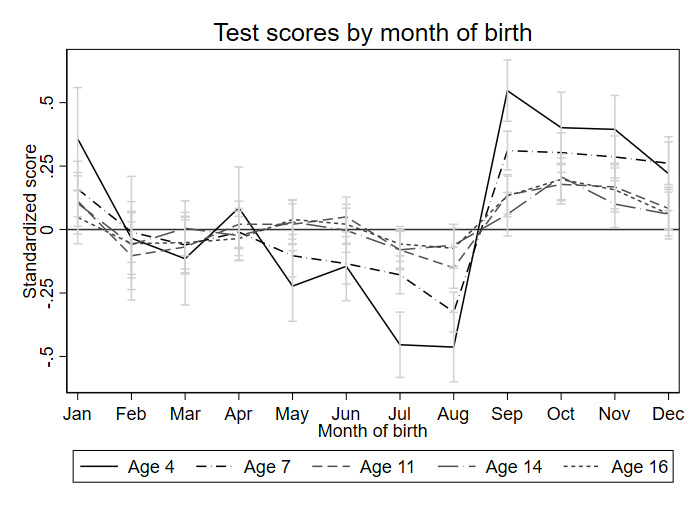
\includegraphics[width=0.6\linewidth]{include/MoB.png}
\label{fig:MoB}
\end{figure}

\autoref{fig:MoB} presents standardized test scores at ages 4-5, 6-7, 10-11, 13-14 and 15-16 as a function of pupils' month of birth. It shows a clear discontinuity in test scores for those born in September and beyond in comparison to those born before September, with the latter group performing significantly worse on all five tests: at age 4-5, those born in September perform approximately one standard deviation better than their August-born peers. This difference reduces as children age (i.e., as the relative difference in age across the cut-off decreases), but it remains sizable and statistically significant across all assessments. Our main interest is in the discontinuity in test scores at the cutoff and in investigating whether (and how) this varies with an individual's genetic predisposition for educational attainment. Thus, in the empirical analyses, we restrict the sample to those born between June and November: three months before and three months after the threshold.\footnote{The three-month bandwidth balances the need for efficiency (including many data points) and the potential of bias (staying close to the cutoff). Our results are robust to different bandwidths (see  \autoref{appsec:robustness}).}  

To explore whether one's month of birth is as good as random, \autoref{tab:descr} reports descriptive statistics for a set of pupil and family characteristics by treatment status. We include only covariates observed before (or at) birth, as any variables measured later in life could be directly or indirectly affected by the treatment. Although \autoref{tab:descr} shows some significant differences, they are very small and do not survive corrections for multiple hypothesis testing. There are also no differences by treatment status in the child's, mother's or father's PGI for education (i.e., there is no evidence of $rGE$; bottom three rows). This suggests that individuals' month of birth is unrelated to the various child and family background characteristics observed here.

\begin{table}[H]
\footnotesize
\caption{\footnotesize Descriptive statistics of child and family characteristics by treatment status.}
\centering
\begin{tabular}{lccccccccccccc}
\toprule
&\multicolumn{3}{c}{Treated} &\multicolumn{3}{c}{Control}           &\multicolumn{1}{c}{\textit{t} test}           \\
& \textit{N} & Mean & & \textit{N} & Mean & & \textit{p} value \\
\midrule
\input include/DescrByTreated
\bottomrule \\
\addlinespace[-2.50ex]
\end{tabular}
\label{tab:descr}
\caption*{\footnotesize \noindent \textit{Notes:} Sample size and means for a set of child and family characteristics observed before or at birth. * denotes a binary variable (0=No;1=Yes). Mother's anxiety and depression scores are sub-scores of the Crown-Crisp Experimental Index, capturing maternal mental health during the pregnancy period. Higher scores mean the mother is more affected. Mother's marital status is equal to one for those ever married (including those widowed, divorced or separated), and zero otherwise. Maternal and paternal education is defined as vocational training, ordinary (O) level, advanced (A) level, and university degree. Social class is defined using the standard UK classification of class based on occupation: professional (I), managerial and technical (II), non-manual skilled (IIInm), manual skilled (IIIm), semi-skilled (IV) and unskilled (V). The last column shows the \textit{p} value from a \textit{t}-test of the difference in means between the treated and control group. }
\end{table}

To more formally check for $rGE$, we explore whether the treated and control groups have systematically different PGIs, which would suggest selection into treatment based on genotype. The top panel of \autoref{fig:kdens_treat_PGI} in \autoref{appsec:MoreTabFig} plots the density of the child's PGI for the treatment and control groups, showing little difference in their distributions. The bottom left and right-hand panels present the PGI for the children's mothers and fathers respectively by treatment and control group, showing similarly overlapping distributions. 
The polychoric correlations between the treatment indicator and the child's PGI ($\rho = -0.013$, s.e. 0.019), the maternal PGI ($\rho = 0.009$, s.e. 0.023), and the paternal PGI ($\rho = -0.021$, s.e. 0.023) are very small and statistically indistinguishable from zero. This suggests there is no gene--environment correlation. 

\subsection{Predictive power of the PGI} \label{sec:PGI}
\autoref{tab:PredictivePower} explores the predictive power of the PGI for the five test scores at different ages. Panel A presents the estimates without controls for the parental PGIs, showing that a one standard deviation increase in the child's PGI is associated with an increase in test scores of 0.163 standard deviations at age 4-5, 0.255 standard deviations at age 6-7 (KS1), and between 0.318 and 0.357 standard deviations at ages 10--16, suggesting that the predictive power of the PGI increases with child age. The PGI explains between 8.5--13.4\% of the variation in test scores.

\begin{table}[H]
\caption{OLS estimates of the effect of the PGIs for EA on test scores at different ages.}
\centering
{\footnotesize
\begin{tabular}{lcccccccccccccccccccc}
\toprule
\input include/PredictivePower_23me_ukb
\bottomrule
\addlinespace[.75ex]
\end{tabular}
\label{tab:PredictivePower}
}
\caption*{\footnotesize \noindent \textit{Notes:} The test score and the polygenic index (PGI) for educational attainment (EA) are standardized to have mean 0 and standard deviation 1 in the analysis sample. All regressions control for gender and the first ten principal components of the genetic data, as well as a dummy if the parental PGIs are missing. Robust standard errors in parentheses. * $p < 0.10$, ** $p < 0.05$, *** $p < 0.01$.}
\end{table}

Panel B of \autoref{tab:PredictivePower} shows the same estimates, additionally adjusting for the maternal and (imputed) paternal PGIs. This shows somewhat smaller, but surprisingly similar, point estimates of the child's PGI, which again increase with child age. The maternal PGI explains additional variation in child test scores, but the paternal PGI does not, except for Key Stage 1. This may be explained by increased measurement error in the paternal PGI due to imputation, but could also reflect that the maternal PGI is more important in shaping child outcomes.\footnote{When we only include the parental PGIs, omitting the child PGI, both the maternal and paternal PGI are highly statistically significant and often of relatively similar magnitude (see \autoref{tab:PredictivePowerApp} in \autoref{appsec:MoreTabFig}).}

\subsection{Functional form} \label{sec:form}
We motivate the functional form used in our main analysis by graphically examining the relationship between the PGI and test scores for our treatment (Sep-Nov borns) and control (Jun-Aug borns) group. We illustrate this with the age 4-5 Entry Assessment. \autoref{fig:PGIxTreat_ea} plots the non-parametric relationship between the PGI and pupils' performance on this test, distinguishing between treatment and control groups. The figure shows that both relationships are positive, with some suggestion that the slope is slightly steeper for the treatment group. Furthermore, the relationship between the PGI and the outcome is approximately linear for both the treatment and control group. We therefore use a linear specification in our main analysis. However, we also explore the robustness of our results to non-linearities in the PGI in \autoref{appsec:robustness}.

\begin{figure}[H]
\centering 
\caption{The relation between PGI Child and the Entry Assessment (age 4-5) test score in the treatment and control group}
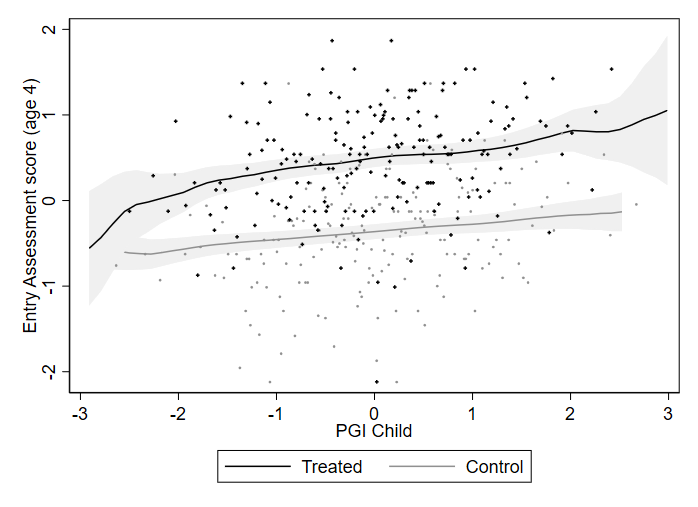
\includegraphics[width=0.6\linewidth]{include/PGSxTreat_ea.png}
\caption*{\footnotesize Note: Black dots refer to the treated group; grey dots to the control group. The polygenic index (PGI) distribution is trimmed to be between -3 and +3 to avoid nonlinear overfitting of outliers.}
\label{fig:PGIxTreat_ea}
\end{figure}

\subsection{Empirical specification} \label{sec:analysis}
We are interested in the discontinuity in test scores between those born before and after September. To estimate the main effect of the PGI ($PGI_i$) and treatment status ($Treated_i$) as well as their interaction, we adopt a standard regression discontinuity design:
\begin{equation}\label{eq:GxE}
\begin{aligned}
        TestScore_i = \delta_0 + & \delta_{G} PGI_i + \delta_{E} Treated_i + \delta_{G \times E} (PGI_i \times Treated_i) + \\ 
        & \delta_1 MoB_i + \delta_2 (MoB_i \times PGI_i) + \delta_3 (MoB_i \times Treated_i) + \\ 
        & \delta_4 (MoB_i \times PGI_i \times Treated_i) + \delta_5\left(X_i,PGI_i,Treated_i\right) + \\
        & \delta_6\left(\sum_{p=1}^{10} PC^p_i,PGI_i,Treated_i\right) + e_i.
\end{aligned}
\end{equation}
where $TestScore_i$ is the test score for child $i$, $PGI_i$ is pupils' EA PGI and $Treated_i$ is the environment of interest: a dummy that equals one for treated individuals and zero for the controls; $MoB_i$ is the running variable, capturing the trend in $TestScore_i$ by month of birth for those born before September (note that this variable runs from -3 to 2, capturing the calendar months June--November, with September set to 0). The coefficients for $MoB_i \times Treated_i $ and $MoB_i \times PGI_i$ capture changes in slope for those born from September onwards and those with higher PGIs respectively. The control variables $X_i$ include a gender dummy, a dummy for birth in 1992 (capturing potential differences in test scores between the birth cohorts), and the first ten principal components of the genetic data ($\sum_{p=1}^{10}PC^p_i$). We also include interactions between the main effects and all (demeaned) controls $X_i$ (represented by $\delta_5(\cdot)$ and $\delta_6(\cdot)$), as suggested by \cite{Keller2014,feigenberg2023omitted}.\footnote{$\delta_5\left(X_i,PGI_i,Treated_i\right)$ denotes all interactions between the demeaned covariates (i.e., gender and year of birth) and $PGI_i$, as well as between the demeaned covariates and $Treated_i$; $\delta_6\left(\sum_{p=1}^{10} PC^p_i,PGI_i,Treated_i\right)$ is shorthand notation for all interactions between the ten demeaned principal components and $PGI_i$ and between the ten demeaned principal components and $Treated_i$.} Hence, the coefficient for $PGI_i$, $\delta_G$, captures the change in test scores associated with a one standard deviation increase in the PGI for the control group ($E=0$) with average characteristics $X_i$, while $\delta_E$ estimates the treatment effect for pupils with a PGI of 0 and average characteristics $X_i$. Finally, $\delta_{G \times E}$ is our estimate of interest, capturing whether the discontinuity in test scores differs by individuals' PGI. 

\autoref{tab:descr} suggests that our environment, i.e., being older in one's grade, is as good as random. This suggests that $\delta_E$ is unbiased (see \autoref{tab:Interpretation}), capturing the causal effect of being older in one's grade on one's test scores. In contrast, since the specification above does not control for the parental genotypes, the PGI potentially captures a spurious correlation with the family environment. To deal with this, we include both the maternal and (imputed) paternal PGIs as additional control variables. In doing so, we additionally control for all interactions between the parental PGIs and $PGI_i$ and between the parental PGIs and $Treated_i$.\footnote{To ensure we keep the same sample as that in \autoref{eq:GxE} (without parental PGIs), we use mean imputation if the parental PGIs are missing and include a dummy to indicate these cases.}

In summary, our setting is rare: the environment is as good as randomly assigned and the data allow for the inclusion of the parental PGIs as covariates to account for parental genetic influences. Random $Treated_i$ ensures $\delta_E$ is unbiased and the inclusion of the parental PGIs ensures $\delta_G$ captures a direct (i.e., causal) genetic effect, removing any genetic nurture or passive $rGE$ effects that enter via the parental genotype. This in turn implies that also $\delta_{G \times E}$ is net of any such influences and captures the causal $G \times E$ effect. Since no sufficiently well-powered parent-child or sibling GWASs exist, the coefficient on $G$ and $G \times E$ is potentially downward biased, though they remain causal effects. 

\subsection{Results} \label{sec:results}
\paragraph{Entering formal schooling:} 
We report the estimated main effects and their interactions for the analysis of the Entry Assessment score in \autoref{tab:MoB_ea}. Columns (1) and (2) present the results from estimating \autoref{eq:GxE}, first without and then with the interaction term. For both specifications, we find that the treatment effect is positive and sizable (1.138 and 1.133, respectively): old-for-grade pupils (born in September -- November) score on average just over one standard deviation higher on their entry test than those who are young-for-grade (born in June -- August). This is consistent with the raw data in \autoref{fig:MoB} where treatment (here roughly the change from August to September) is about 1 standard deviation. Furthermore, our estimates suggest that among the controls, being born one month later (MoB) is associated with a 0.148 standard deviation reduction in the average test score; this trend is slightly less pronounced (though insignificantly so) for the treated (differing from 0.148 by a statistically insignificant 0.055). The PGI coefficient in column (1) suggests that a one standard deviation increase in the EA PGI is associated with an increase of 0.156 standard deviations in the Entry Assessment score---a result similar to the average predictive power of the PGI of 0.163 in \autoref{tab:PredictivePower}.

Considering the $G \times E$ estimate (Treated $\times$ PGI Child) in Column (2), we find that the discontinuity in the entry assessment score by treatment status is larger for those with a higher PGI: a one standard deviation increase in the PGI is associated with an additional 0.088 standard deviation increase in the discontinuity. This is consistent with the descriptive analysis of \autoref{fig:PGIxTreat_ea}, showing a steeper line in the treatment versus the control group. Taken at face value, the regression results suggest that a delayed entry-age increases skill inequalities at ages 4-5 (i.e., before the start of formal schooling) associated with genetic endowments, although the effect is only marginally significant at the 10\% level.

We next show the estimates that account for the parental PGIs as well as interactions between the parental PGIs and $G$ and between the parental PGIs and $E$: our preferred specification. In line with the prediction from \autoref{tab:Interpretation}, compared to Column (2), the effect of the treatment remains roughly similar while the effect of the EA PGI decreases in Column (3). The results show that our main effect of interest $\hat{\delta}_{G \times E}$ increases both in size and in precision when including the parental PGIs and their interactions with PGI Child and Treated (0.126, s.e. 0.021, $p < 0.01$), suggesting that the interaction effect in column (2) is unlikely to be driven by genetic nurture or passive $rGE$.

\begin{table}[H]
\caption{OLS estimates of the main and interaction effects of being old-for-grade (Treated) and the EA PGI on children's Entry Assessment (age 4-5) test score, with and without controls for parental PGIs.}
\centering
{\scriptsize
\begin{tabular}{lcccccccccccccccccccc}
\toprule 
\input include/MoB_ea
\bottomrule
\addlinespace[.75ex]
\end{tabular}
\label{tab:MoB_ea}
}
\caption*{\footnotesize \noindent \textit{Notes:} The analysis uses a bandwidth of 3 months before and after the September cutoff (i.e., June till November). Additional control variables include gender, year of birth, the first 10 principal components, a dummy for missing parental PGI, and interactions of all covariates with PGI Child and with Treated. Robust standard errors in parentheses, clustered by month of birth. * $p < 0.10$, ** $p < 0.05$, *** $p < 0.01$.}
\end{table}

\paragraph{Progressing through formal schooling:}
To explore how the $G \times E$ effect changes as children age and progress through the formal schooling system, \autoref{tab:MoB_ks} shows the analysis that uses the four Key Stage tests as the outcomes of interest.  
The main ``treatment effect'' is consistent with the previous literature: those who are older in their grade have test scores that are approximately 0.7, 0.4, 0.2, and 0.3 standard deviations higher at ages 6-7, 10-11, 13-14, and 15-16 respectively; the treated perform better than the controls on all Key Stage tests, though the difference declines as children age. The downward trend in test scores by month of birth (MoB) is also visible in all specifications and is less steep for those born after September. Focusing on the $G \times E$ interaction term (Treated $\times$ PGI), we find a \textit{negative} effect that is significant across all Key Stages other than Key Stage 3, where the coefficient is close to zero. This finding suggests that although the treated have higher test scores on average, the discontinuity is \textit{smaller} for those with a higher PGI. In other words, the benefits of delayed entry on test performance are larger for those with lower PGIs.  Our preferred specification however, is one that controls for the parental PGIs and its interactions. We find that our estimates are generally robust to their inclusion (the even columns). One exception is the KS1 assessment, for which adding these extra controls increases the standard error on the $G \times E$ interaction term substantially and prevents us from rejecting the null.  However, even here the point estimate is consistent with estimates from specifications omitting these controls. In fact, adding these controls \textit{increases} the magnitude of the estimate.

The estimated interactions, summarized in \autoref{fig:coefplot}, are economically meaningful. For example, for Key Stage 4 we find an average treatment effect of 0.27-0.28 standard deviations associated with being assigned to old-for-grade. The estimated interaction between treatment and the PGI suggests that two children with a one standard deviation difference in the EA PGI are expected to have differences in this treatment effect of 0.04 - 0.05 standard deviations, or 15-20\% of the overall treatment effect. In \autoref{appsec:robustness} we investigate the robustness of the results with respect to non-linearities in the PGI and the chosen bandwidth of our RDD. The results remain very similar in terms of magnitude, sign, and significance. When allowing for non-linearities in addition to an extensive set of interaction terms, precision is considerably reduced -- occasionally increasing \textit{p}-values above commonly employed thresholds for statistical significance. However, even then the sign and magnitude remain very similar to our main results. 

\begin{table}
\caption{OLS estimates of the main and interaction effects of being old-for-grade (Treated) and the EA PGI on children's Key Stage test scores.}
\centering
{\scriptsize
\begin{tabular}{lcccccccccccccccccccc}
\toprule
\input include/MoB_other
\bottomrule
\addlinespace[.75ex]
\end{tabular}
\label{tab:MoB_ks}
}
\caption*{\scriptsize \noindent \textit{Notes:} The analysis uses a bandwidth of 3 months before and after the September cutoff (i.e., June till November). Additional control variables include gender, year of birth, the first 10 principal components, a dummy for missing parental PGI, and interactions of all covariates with PGI Child and with Treated. Robust standard errors in parentheses, clustered by month of birth. * $p < 0.10$, ** $p < 0.05$, *** $p < 0.01$.}
\end{table}

\subsection{Interpretation and discussion} \label{sec:interpret}

Our estimates of the treatment effect and the PGI are in line with the existing literature.
We estimate that being old-for-grade has positive main effects across all available test scores: individuals assigned a later age of school entry have an educational advantage relative to their younger peers. This effect declines in magnitude for later grades, perhaps reflecting a decline in the relative age differences between treated and untreated students as they all grow older.  Unsurprisingly, children with higher EA PGIs also have an advantage, and the magnitude of the main PGI effect appears to be relatively stable across grades. 

The $G\times{}E$ interactions may seem more surprising. They are qualitatively different when considering performance on the Entry Assessment test taken before school entry (ages 4-5) compared to performance on the four Key Stage assessment tests taken as pupils progress through the schooling system (ages 7-16). Being older at school entry benefits children on the Entry Assessment test (ages 4-5), but more so for those with a higher genetic propensity for education, exacerbating genetic inequalities. By contrast, while being old-for-grade also benefits children on the assessment tests at later ages (ages 7-16), it benefits those with a lower genetic propensity for education more, reducing genetic inequalities. This qualitative difference in the $G\times{}E$ interaction suggests an interesting role of the formal schooling system in reducing genetic inequality.  Here we put forward an interpretation of our results given the theory outlined in \hyperref[sec:econModel]{Section~\ref*{sec:econModel}}. While speculative, this exercise highlights the potential value of incorporating economic theory into $G\times{}E$ studies.

The positive $G\times{}E$ interaction for the Entry Assessment test is in line with the broader literature on parental investment in skill formation. Children benefit both from a higher genetic propensity and from being older at school entry. This literature stresses the existence of complementarities between inputs, including between parental investments and past skills \citep[e.g.,][]{cunha2007technology,Cunha2010,Muslimova2020b}.  Sources of advantage tend to compound one another and magnify inequality. This makes the negative interactions for the Key Stage tests, taken after teachers start investing in children's human capital,  more surprising and of interest for public policy.  Students with lower EA PGIs experience greater gains on the Key Stage tests from being old-for-grade. 
These opportunities for substitutability emerge within the formal schooling system, and may mitigate disparities arising from genetic factors and differences in pre-entry skills. 
Data on teacher-child interactions would allow us to understand the interplay within the classroom and thereby explore potential mechanisms for our findings. Unfortunately ALSPAC does not contain such data.

Nevertheless, our collection of results can still shed light on the signs and magnitudes of the  mechanisms by which genotype and age-at-entry interact to influence later Key Stage test scores. Consider mechanism (1) from \autoref{eqn:GxEModel}: differential pre-entry skill accumulation, formalized as $\frac{\partial \theta_{i}^\tau}{\partial \theta_{i}^e}\left(\theta_{i4}^{e}, G_{i}, 4\right) \left[\frac{d \theta_{i 5}^{e *} }{d G_i}- \frac{d \theta_{i 4}^e}{d G_i}\right]$.  Since we observe entry skills $\theta_{i}^{e}$ through the Entry Assessment, we directly evaluate this mechanism in \autoref{tab:MoB_ea}, where we find that being old-for-grade benefits those with a high PGI more on the entry test (Treated $\times$ PGI Child is positive, 0.126 [column 3]),  implying that $\frac{d \theta_{i 5}^{e *} }{d G_i}- \frac{d\theta_{i 4}^e}{d G_i}$ is positive. Assuming entry skills positively influence later skills ($\partial \theta_{i}^\tau/{\partial \theta_{i}^e}>0$), and ignoring other drivers, mechanism (1) should generate a positive $G\times{}E$ interaction in the later Key Stage tests, $\theta_{i}^\tau$. The fact that we estimate a negative $G\times{}E$ interaction suggests that the other three mechanisms (2, 3 and 4) collectively generate a sufficiently strong negative interaction to more than offset differential pre-entry skill accumulation.  

Consider mechanism (3): entry skill--gene interaction: $\frac{\partial^2 \theta_{i}^\tau}{\partial G_i \partial \theta_{i}^e}\left(\theta_{i 4}^{e}, G_{i}, 5\right)\left[\theta_{i 5}^{e*}-\theta_{i 4}^e\right]$.  Since being old-for-grade positively impacts entry skills, $\theta_{i 5}^{e*}>\theta_{i 4}^e$, this mechanism would be consistent with our finding  if the productivity of entry skills were lower for individuals with higher PGIs, $\frac{\partial^2 \theta_{i}^\tau}{\partial G_i \partial \theta_{i}^e}\left(\theta_{i 4}^{e}, G_{i}, 5\right) < 0$. One (imperfect) way to evaluate this is to control for entry skills and its interaction with the PGI in our regressions. If mechanism (3) were negative, adding these controls would make the $G\times E$ interaction coefficient more positive. 

We perform this exercise in  \autoref{tab:mechan_ea} where, for each Key Stage test, we present three specifications. The first column repeats the specification found in \autoref{tab:MoB_ks} with our full control set (including parental PGIs) as a baseline.  The second column repeats this specification, but restricts the sample to the set of children for whom we observe non-missing values of the age 4-5 entry assessment.  The third column adds a control for the entry assessment score, and an interaction between the entry assessment score and the PGI. These tests are not perfect. First, sample sizes drop substantially when restricting the sample to the subset for which we have Entry Assessment scores. More importantly, the Entry Assessment score, and its interactions with the EA PGI, are endogenous, which makes it difficult to interpret the $G\times{}E$ coefficient after controlling for these regressors. Comparing the second and third column in \autoref{tab:mechan_ea}, the additional controls, if anything, make the  interaction effects more negative. Moreover, we find no evidence of statistically significant interactions between entry skills and the PGI, casting doubt on mechanism (3) as an important driver of our results. Hence, while we caution the reader not to over-interpret these regressions, we consider them suggestive. 

Since mechanism (1) should generate a positive interaction, and mechanism (3) does not appear to be important, we are left with mechanisms (2) and (4). Our data do not allow us to separate mechanisms (2) and (4), nor do they allow us to draw firm conclusions about how these mechanisms operate in our specific context.  Nevertheless, we can offer some speculative possibilities. Since higher PGI students on average tend to have higher entry skills, $\left(\frac{d\theta^{e*}_{i5}}{d G_i}>0\right)$, mechanism (2) could explain our results if being old-for-grade reduces the marginal productivity of entry skills in the production function in a way that disadvantages individuals with higher PGIs:  $\left[\frac{\partial \theta_{i}^\tau}{\partial \theta_{i}^e}\left(\theta^{e*}_{i 5}, G_{i}, 5\right)-\frac{\partial\theta_{i}^\tau}{\partial \theta_{i}^e}\left(\theta^e_{i 4}, G_i, 4\right)\right] < 0$.
Higher PGI children might have higher entry skills, but this could matter less among those who are old-for-grade.  
On the other hand, mechanism (4), $\frac{\partial \theta_{i}^\tau}{\partial G_i}\left(\theta^e_{i 4}, G_{i,}, 5\right)-\frac{\partial \theta_{i}^\tau}{\partial G_i}\left(\theta^e_{i 4}, G_i, 4\right)$, can explain our results if being old for grade reduces the relationship between the genetic component and skill accumulation while in school for the same level of entry skills. 

Mechanisms (2) and (4) are similar because they both show how age can compensate for other factors in skill development at school, serving as a substitute for either initial skills or genetic endowments.
A speculative but illustrative example could involve relational maturity -- older children could be more mature or confident in ways that allow them to better ask for help, or extract assistance from teachers or peers. Among old-for-grade children, this might offset advantages that students have from genetic endowments in formal schooling.  Children with low PGIs who are old-for-grade may thus be able to more easily catch-up with their peers if they start at a skills deficit. Another possibility is that teachers may target their time and attention in the classroom on those who are falling behind. 
Indeed, a potentially important feature of the UK institutional education setting is the fact that children do not repeat school years. Hence, to ensure that all children reach the minimum required standard to progress to the next year, teachers will spend more time with lower-performing students. Since these are more likely to be August-borns and low-PGI pupils (who on average perform worse on educational tests), our negative $G \times E$ effects are consistent with the existence of complementarities between genetic endowments and teacher inputs. This also means that our findings may be specific to our setting; it will be interesting to explore whether they replicate in other educational systems.

Whatever the specific micro-foundations, it is noteworthy that these opportunities for substitutability emerge within the formal schooling system. Under the right conditions (e.g., when children are older at entry), the instruction and personal interactions provided by the formal schooling system may work to mitigate disparities arising from genetic factors and differences in pre-entry skills. 
Such possibilities may not be obvious from the existing literature, which stresses complementarities between endowments and early, pre-schooling skills.  Our findings are, however, consistent with those of \citet{arold2022genetic} and \citet{cheesman2022genes}, who find that children with lower EA PGIs benefit more from high quality teachers and schools. Taken together, these findings provide a fruitful area for future theoretical and empirical research on differential interactions between endowments and investments in the home versus school setting.

Depending on policy preferences regarding equity and efficiency, our finding that children with lower PGIs appear to gain the most from delaying entry into formal schooling provides important information to set school entry age policies and determine appropriate public funding for preschools. More speculatively, one could also think in terms of the targeting of interventions or school policies. In many school systems, families have some control over when their children enter the formal schooling system. Indeed, if the ALSPAC cohort were starting school now, families with children born between April 1 and August 31 could decide to hold them back a year. In such settings, individual families on the margin might use privately acquired genetic test results to help guide the decision about when to have a child enter formal schooling.  It is certainly not clear that the magnitudes of the interactions we find would make genetic information useful for this purpose, particularly given the current limitations on using genetic data for \textit{individual}-level prediction of outcomes such as educational attainment \citep{morris2020can}. However, whether a particular effect size is large depends on the preferences, risk-tolerances, and expectations of individual families. 


\begin{landscape}
\begin{table}
\caption{OLS estimates of the main and interaction effects of being old-for-grade (Treated) and the EA PGI on children’s Key Stage test scores, controlling for Entry Assessment.}
\centering
{\scriptsize
\begin{tabular}{lcccccccccccccccccccc}
\toprule
\input include/mechan_ea
\bottomrule
\addlinespace[.75ex]
\end{tabular}
\label{tab:mechan_ea}
}
\caption*{\scriptsize \noindent \textit{Notes:} The analysis uses a bandwidth of 3 months before and after the September cutoff (i.e., June till November). The models include parental PGIs. Additional control variables include gender, year of birth, the first 10 principal components, a dummy for missing parental PGI, and interactions of all covariates with PGI Child and with Treated. Robust standard errors in parentheses, clustered by month of birth. * $p < 0.10$, ** $p < 0.05$, *** $p < 0.01$. The first column in each set of results reproduces the final specification in \autoref{tab:MoB_ks}; the second column includes the same specification but in the sample with non-missing Entry Assessment (age 4-5) scores; the third column controls for Entry Assessment and its interaction with PGI Child.}
\end{table}
\end{landscape}

\section{Conclusion} \label{sec:discussion}
Recent advances in the collection and processing of genetic data have created new opportunities for improving our understanding of how nature and nurture interact in shaping individual outcomes, illuminating some of the oldest questions in the social sciences from a new angle. 
Economists can benefit from these advances, even if they are not interested in genetic effects. This is because $G \times E$ analyses can (i) assess treatment effect heterogeneity, (ii) test theoretical predictions, and (iii) uncover economic, social and behavioral mechanisms. We demonstrated best practice in a study of $G \times E$ interplay, examining interactions between one's age at school entry and one's genetic propensity for educational attainment. Our results suggest (previously unobserved) differential productivity by child genotype, where children with a lower genetic propensity for education benefit more in terms of their test scores from delayed school entry. 

Our empirical application is one of few studies (see \autoref{tab:Examples} in \autoref{appsec:MoreTabFig}) exploiting random variation in both genotype and environment, enabling causal inferences in both $G$ and $E$. While this is an important contribution on its own, our extensive methodological review also illustrates the power of interdisciplinary research. Combining approaches from genetics with its focus on the estimation of causal genetic effects, and economics with its focus on causal environmental effects, allows for what we consider the ``ideal experiment''. In this ideal experiment, randomized variation in genotype (ideally based on a within-family GWAS) is combined with quasi-random variation in the environment.

Governments are investing heavily in large biobanks for research. The UK Biobank (${\sim}$500,000 genotyped individuals) has been available for some years, and next-generation biobanks such as the All of US in the United States and Our Future Health in the UK are ambitiously building biobanks of, respectively, one and five million individuals. These datasets will alter the playing field of future GWASs, increasing the number of outcomes for which genetic data explains a substantial part of its variation. These data collection efforts will also increase the availability of genetic data from relatives, allowing for well-powered within-family GWASs. This would pave the way for the ``ideal experiment''. 

There are ethical issues involved in working with genetic data and researchers have obligations to preserve the highest standards of privacy, confidentiality, and responsible communication. Researchers must also take seriously the need to help the public understand how to interpret research findings based on genetic data and to clarify what conclusions can and cannot be drawn \citep{dangerouswork}. We would argue that the potential uses of genetic data carry societal implications and associated risks, but simply denying the existence of genetic differences across individuals is unlikely to be the right solution \citep{raffington2020polygenic,Harden2021}. Research in economics and the social sciences on $G \times E$ interplay can help identify causal pathways involved in individual development and refute genetic or environmental determinism while identifying policy-relevant environments that can reduce socioeconomic or genetic inequalities. In doing so, it may help improve the well-being of the population. 

\section{Data availability statement} \label{sec:dataavailability}
The code to reproduce this article is available on Zenodo at \url{https://zenodo.org/records/14968164}.

The data used in this study is the Avon Longitudinal Study of Parents and Children (ALSPAC). Due to confidentiality agreements, access to ALSPAC data must be requested directly from the data providers (University of Bristol). Details on data access can be found at: \url{https://www.bristol.ac.uk/alspac/}.

\newpage
\begin{spacing}{1.0}
\setlength{\bibsep}{0.0pt}
\putbib[genes]
\end{spacing}
\end{bibunit}

\clearpage

\section*{Acknowledgments}
We thank the \href{https://gene-environment.com/}{GEIGHEI} and \href{https://essgn.org/}{ESSGN} members for many discussions on $G \times E$ interplay and, in particular, Rita Dias Pereira for creating the polygenic indices used in this study. We gratefully acknowledge financial support from NORFACE DIAL (462-16-100). Research reported in this publication was also supported by the European Research Council (DONNI 851725 and GEPSI 946647), the European Union’s Horizon 2020 research and innovation programme under the Marie Skłodowska-Curie grant agreement (ESSGN 101073237), the National Institute on Aging of the National Institutes of Health (RF1055654, R56AG058726, R01AG078522, and R01AG079554), and the Dutch National Science Foundation (016.VIDI.185.044).  The UK Medical Research Council and Wellcome (217065/Z/19/Z) and the University of Bristol provide core support for ALSPAC. This publication is the work of the authors who will serve as guarantors for the contents of this paper. A comprehensive list of grants funding is available on the ALSPAC website (http://www.bristol.ac.uk/alspac/external/documents/grant-acknowledgements.pdf). GWAS data was generated by Sample Logistics and Genotyping Facilities at Wellcome Sanger Institute and LabCorp (Laboratory Corporation of America) using support from 23andMe. Consent for biological samples has been collected in accordance with the Human Tissue Act (2004). We are extremely grateful to all the families who took part in this study, the midwives for their help in recruiting them, and the whole ALSPAC team, which includes interviewers, computer and laboratory technicians, clerical workers, research scientists, volunteers, managers, receptionists and nurses. Ethical approval for the study was obtained from the ALSPAC Ethics and Law Committee and the Local Research Ethics Committees. Informed consent for the use of data collected via questionnaires and clinics was obtained from participants following the recommendations of the ALSPAC Ethics and Law Committee at the time.
\clearpage
\appendix

\begin{bibunit}

\renewcommand{\thetable}{A.\arabic{table}}
\renewcommand{\thefigure}{A.\arabic{figure}}
\renewcommand{\theequation}{A.\arabic{equation}}
\setcounter{table}{0} 
\setcounter{figure}{0} 
\setcounter{equation}{0} 

\section{Glossary}
\label{appsec:glossary}

In this section, we provide an overview of the genetic terms and concepts used in the paper. 

\bigskip 
\textbf{Active gene--environment correlation:} An association between genetic variation and an environment resulting from self-selection of genetically different individuals into particular environments.

\textbf{Alleles:} The nucleotides that can be present at a specific location in DNA.

\textbf{Base pairs:} Nucleotides are paired: ``A'' on one strand of the DNA always binds with ``T'' on the other strand, and ``C'' always binds with ``G''. These combinations are called base pairs.

\textbf{Candidate gene:} A polymorphism hypothesized to be associated with a particular phenotype.

\textbf{Chromosome:} A long DNA molecule. Every cell in the human body contains 23 pairs of chromosomes (22 so-called autosomal chromosomes and 1 sex chromosome). One of each pair is inherited from the mother and the other from the father.

\textbf{Copy Number Variant (CNV):} A type of genetic variation that refers to the duplication or deletion of a specific segment of DNA in an individual's genome. These variations can range in size from a few base pairs to large stretches of DNA encompassing multiple genes. 

\textbf{DNA:} Human deoxyribonucleic acid (DNA), the sequence of about 3 billion pairs of nucleotide molecules. Its double-helix structure joins two strands of DNA, where the nucleotide ``A'' binds with ``T'', and ``G'' binds with ``C''.

\textbf{Evocative gene--environment correlation:} An association between genetic variation and an environment resulting from an environmental reaction to genetic differences.

\textbf{Epigenetics:} The study of heritable phenotypic variation that does not involve changes in the DNA sequence of nucleotides.

\textbf{Gene--environment correlation:} An association between genetic variation and an environment.

\textbf{Gene:} A sequence of nucleotides in the DNA that encodes for a particular protein or proteins.

\textbf{Genetic nurture:} Parental genes influencing offspring outcomes through environmental pathways.

\textbf{Genetic variation:} Differences in the DNA among individuals; copy-number variants (CNV) and single-nucleotide polymorphisms (SNPs) constitute the most common source of genetic variation.

\textbf{Genotype:} The complete set of genetic material. It can, however, also refer to the specific combination of base pairs (in a chromosome pair) at a particular location in the DNA sequence. If the base pairs are the same, the genotype is homozygous. If they are different, it is heterozygous.

\textbf{Genome-wide association study (GWAS):} A study in which millions of polymorphisms from the whole genome are individually tested for association with a phenotype.

\textbf{GWAS meta-analysis:} Meta-analysis of genome-wide association study (GWAS) results from different samples.

\textbf{Genome-wide significance:} The significance level at which an association is considered statistically significant in a genome-wide association study (GWAS) ($5\times10^{-8}$).

\textbf{G$\times$E interplay:} The interplay between people’s genotype and the (e.g., social, biological, and economic) environment in which they live contributing to intra-individual differences.

\textbf{Heritability:} The proportion of the total variance in a phenotype that can be explained by genetic factors.

\textbf{Imputation:} Imputation of not directly genotyped genetic variation from reference panels based on linkage disequilibrium (LD).

\textbf{Linkage disequilibrium (LD):} The correlation between adjacent nucleotides in the DNA resulting from the co-inheritance of alleles.

\textbf{Locus:} A stretch of nucleotides in strong linkage disequilibrium (LD) with each other.

\textbf{Major allele:} The allele of a single-nucleotide polymorphism (SNP) that is most common in the population.

\textbf{Manhattan plot:} A plot often used to visualize genome-wide association study (GWAS) results, with genomic coordinates on the $x$ axis and the negative logarithm of the associated $p$ value for each SNP on the $y$ axis. An example is \autoref{fig:manhattan}.

\textbf{Minor allele:} The allele of a single-nucleotide polymorphism (SNP) that is least common in the population.

\textbf{Nucleotide:} The basic component molecules of DNA. Human DNA is composed of a sequence of about 3 billion pairs of nucleotide molecules. There are four different nucleotides in the DNA: adenine (A), guanine (G), cytosine (C) and thymine (T).

\textbf{Passive gene--environment correlation:} An association between people's genetic makeup and an environment resulting from the correlation between parental genes and the environment in which the child is raised.

\textbf{Phenotype:} An observable trait of an organism.

\textbf{Pleiotropy:} One gene/genetic variant influencing more than one phenotype.

\textbf{Polygenic index:} The best linear genetic predictor of a phenotype, constructed as the linear combination of single-nucleotide polymorphisms (SNPs) weighted by their association with the phenotype as estimated in a genome-wide association study (GWAS). It also also referred to as polygenic score.

\textbf{Polygenic trait:} A trait influenced by many genetic variants, with each having a small effect.

\textbf{Polymorphism:} Locations in the DNA where the nucleotides differ between individuals.

\textbf{Population stratification:} The presence of a systematic difference in allele frequencies between subpopulations within a population.

\textbf{Principal components:} Principal components extracted from the genetic relatedness matrix; can be used to control for subtle population stratification.

\textbf{Single-nucleotide polymorphism (SNP):} A single nucleotide location in the DNA that varies between individuals.

\clearpage
\renewcommand{\thetable}{B.\arabic{table}}
\renewcommand{\thefigure}{B.\arabic{figure}}
\renewcommand{\theequation}{B.\arabic{equation}}
\setcounter{table}{0} 
\setcounter{figure}{0} 
\setcounter{equation}{0} 

\section{Primer on genetics} 
\label{appsec:genes}
\subsection{Genetics in a nutshell}
Human DNA is composed of sequences of approximately 3 billion pairs of nucleotide molecules. These nucleotides come in four varieties: adenine (A), guanine (G), cytosine (C) and thymine (T). The nucleotides together constitute the genome. The human genome is divided into 23 pairs of chromosomes (22 autosomal chromosomes and 1 sex chromosome), where for each pair, one chromosome is inherited from the mother and one from the father. Each chromosome contains a single double-stranded piece of DNA. ``A'' on one strand is always paired with ``T'' on the other strand, and ``C'' is always paired with ``G''. These combinations are called base pairs, and stretches of these pairs coding for a protein are called genes. The human genome consists of around 25,000 genes that code for proteins with a specific function \citep{sequencing2004finishing}. In addition, there are regions in-between genes with important regulatory functions. 

Most nucleotides ($\sim$99.9\%) in human DNA are identical from person to person. The part of DNA where people are different from each other are called polymorphisms; the location of most polymorphisms is well known by now. For many applications, it is therefore not necessary to sequence each individual's full genome. The most common polymorphisms are Copy Number Variants (CNVs)---genetic variations involving duplications or deletions of DNA segments---and Single Nucleotide Polymorphisms (SNP)--- one-letter variations at a single-nucleotide locus. These variants of nucleotides are called alleles. In the human genome, there are approximately 85 million SNPs with a minor allele (i.e., the less common allele) frequency of $>1\%$ \citep{1000Genomes2015}. Current genotyping arrays measure several million of these SNPs, and many more that are not measured (typically $>$40 million) can be imputed with high accuracy because of the correlation structure in the genome \citep[so-called linkage disequilibrium,][further explained below]{reich2001linkage} and the availability of large reference panels \citep{quick2019sequencing}. 

\subsection{Genome-wide association studies}
\label{appsec:gwas}
The polygenic nature of most traits was established through genome-wide association studies (GWASs). In a GWAS, one tests for associations between $J$ genetic variants (SNPs) and an outcome of interest without restricting the set of SNPs on theoretical grounds. Specifically, an ideal GWAS relates all SNPs ($G_{ij}$, coded as 0, 1, or 2, reflecting the number of minor alleles) to a specific outcome ($Y_i$) for individual $i$ in a regression framework of the form
\begin{eqnarray}
Y_i = \sum_{j=1}^{J} \beta_j G_{ij} + \mathbf{x}_i^{'} \zeta + \varepsilon_i,
\label{eq:gwas}
\end{eqnarray}
with SNP effects $\beta_j$, relevant controls $\mathbf{x}_i$, and an error term $\varepsilon_i$. In practice, however, this ideal model cannot be identified since existing datasets cover fewer individuals than SNPs \citep{Benjamin2011}.\footnote{At the time of writing, the biggest sample size of a GWAS is 5.4 million \citep{Yengo2022}.} 
GWASs therefore consider all $J$ SNPs by running sequential regressions for each SNP at a time. Thus, in its most basic form, a GWAS regresses the outcome of interest on a single SNP $j$ and repeats this procedure $J$ times, once for each SNP: 
\begin{eqnarray}
Y_i = \beta_j^{GWAS} G_{ij} + \mathbf{x}_i^{'} \zeta_j + \varepsilon_{ij}.
\label{eq:gwas2}
\end{eqnarray}
This produces a list of $\beta_j^{GWAS}$ coefficients for all $J$ SNPs. The set of control variables $\mathbf{x}_i$ is usually very sparse, typically including age and sex alongside the first (usually ten) principal components (PCs) of the genetic data to account for population stratification \citep{Price2006}.\footnote{\label{fn:popstrat} Population stratification is a form of confounding where the genetic makeup of ancestors influences one's genetic makeup as well as the outcome through nongenetic pathways (see also \autoref{appsec:glossary}). More specifically, if a population is stratified into subpopulations that do not mate randomly and an outcome happens to be more common in one subpopulation for non-genetic reasons, then the outcome will appear to be correlated with any SNPs that also happen to be more common in that sub-population. A commonly used hypothetical example is the ``chopstick gene'' \citep{hamer2000beware}, where people of Asian descent have different allele frequencies and tend to eat with chopsticks for cultural reasons. A GWAS investigating the genetic basis of chopstick use without controlling for ancestral differences in allele frequencies would then pick up a ``chopstick gene''. By conditioning on principal components, the researcher essentially compares individuals within a common lineage and from the same genetic pool. For this reason, it is not necessary to include principal components in a within-family analysis.} Importantly, due to the sparsity of control variables and the correlation between closely spaced SNPs, $\beta_j^{GWAS}$ is not necessarily equal to $\beta_j$.

The set of $\beta_j^{GWAS}$ coefficients is a simple linear projection of the outcome of interest on the space spanned by the measured SNPs. Imposing linearity neglects any form of interaction, whether gene--gene or gene--environment, thereby estimating a weighted average of the SNP-outcome associations over multiple environments \citep[e.g.,][]{loken2012linear}. The consequences for the resulting $PGI \times E$ interaction term are discussed in \hyperref[sec:missp]{Section~\ref*{sec:missp}}.

Running so many regressions requires a correction for multiple hypothesis testing. Considering that there are $\sim$1 million approximately independent blocks of SNPs in the human genome (adjacent SNPs are often in linkage disequilibrium, i.e., inherited together), the commonly used criterion for genome-wide statistical significance is $p <5 \times 10^{-8}$ (i.e., 0.05 divided by 1,000,000). The stringent significance level, in combination with the tiny effect sizes of individual SNPs on outcomes \citep{Rietveld2013,Chabris2015}, necessitates the use of extremely large samples to ensure adequate power. Legal and privacy reasons usually prohibit the joint analysis of genetic datasets. For this reason, researchers typically pursue a meta-analysis strategy to obtain a sufficiently large discovery sample \citep{Visscher2017}. Consortia such as the Social Science Genetic Association Consortium (SSGAC), Genetic Investigation of ANthropometric Traits (GIANT) and GWAS \& Sequencing Consortium of Alcohol and Nicotine Use (GSCAN) have been key to this, coordinating the analyses (i.e., harmonizing the outcomes, quality-controlling consortium datasets) and bringing together the results of large numbers of smaller datasets. In such meta-analyses, only GWAS summary results (the effect sizes for each SNP) are shared between consortium members, addressing the legal and privacy barriers to their joint use. 
The GWAS meta-analysis approach has made possible an unprecedented surge in genetic discoveries that replicate consistently \citep{Visscher2017}.\footnote{By contrast, so-called candidate-gene studies, a hypothesis-driven approach, have weak replication records \citep[see e.g.,][]{Hewitt2012,Chabris2013}. } 

GWAS results are typically presented using so-called Manhattan plots. As an example, \autoref{fig:manhattan} provides the Manhattan plot visualizing the results of the second GWAS of educational attainment \citep{okbay2016}. The $x$-axis of the Manhattan plot represents the position of the SNP in the genome (the numbers 1-22 reflect the autosomal chromosomes) and the $y$-axis the strength of the evidence for an association with the outcome variable (as reflected in the $p$ value). The $p$ value is transformed (by taking the negative of the 10 log of the $p$ value) so that higher values represent stronger associations. Specifically, when a dot (representing a single SNP) is above the dashed line in the Manhattan plot (note that –log$_{10}(5\times10^{-8}) = 7.3$), the SNP is genome-wide significant. The Manhattan plot also visualizes the effect of linkage disequilibrium. Because SNPs physically close to one another are more likely to be inherited together (i.e., are in linkage disequilibrium), the regression results are very similar for adjacent SNPs. As a result, $p$ values of adjacent SNPs are highly correlated. This is visible in the towers of dots around genome-wide significant SNPs. The result looks like the skyscrapers of Manhattan towering above lower-level buildings.

Because of linkage disequilibrium, each genome-wide significant SNP is correlated with adjacent SNPs. Each block of correlated SNPs is called a genome-wide significant locus. One typically picks a lead SNP: the SNP in a genome-wide significant locus with the smallest $p$ value. By construction, the set of lead SNPs are therefore approximately uncorrelated with each other. The first GWAS meta-analysis of educational attainment used a combined sample of $\sim$125,000 people \citep{Rietveld2013} and identified 3 genome-wide significant loci. The second GWAS of educational attainment used a sample of $\sim$400,000 people \citep{okbay2016} and identified 74 genome-wide significant loci. The third, \cite{lee2018gene}, used a sample of $\sim$1.1 million individuals to uncover 1,271 lead SNPs, and the fourth GWAS of educational attainment used $\sim$3 million individuals and identified 3,952 lead-SNPs associated with educational attainment \citep{Okbay2022}. This rapid growth in the power of genetic discovery exemplifies the genetics revolution that we are in the midst off. 

\begin{figure}
    \centering
    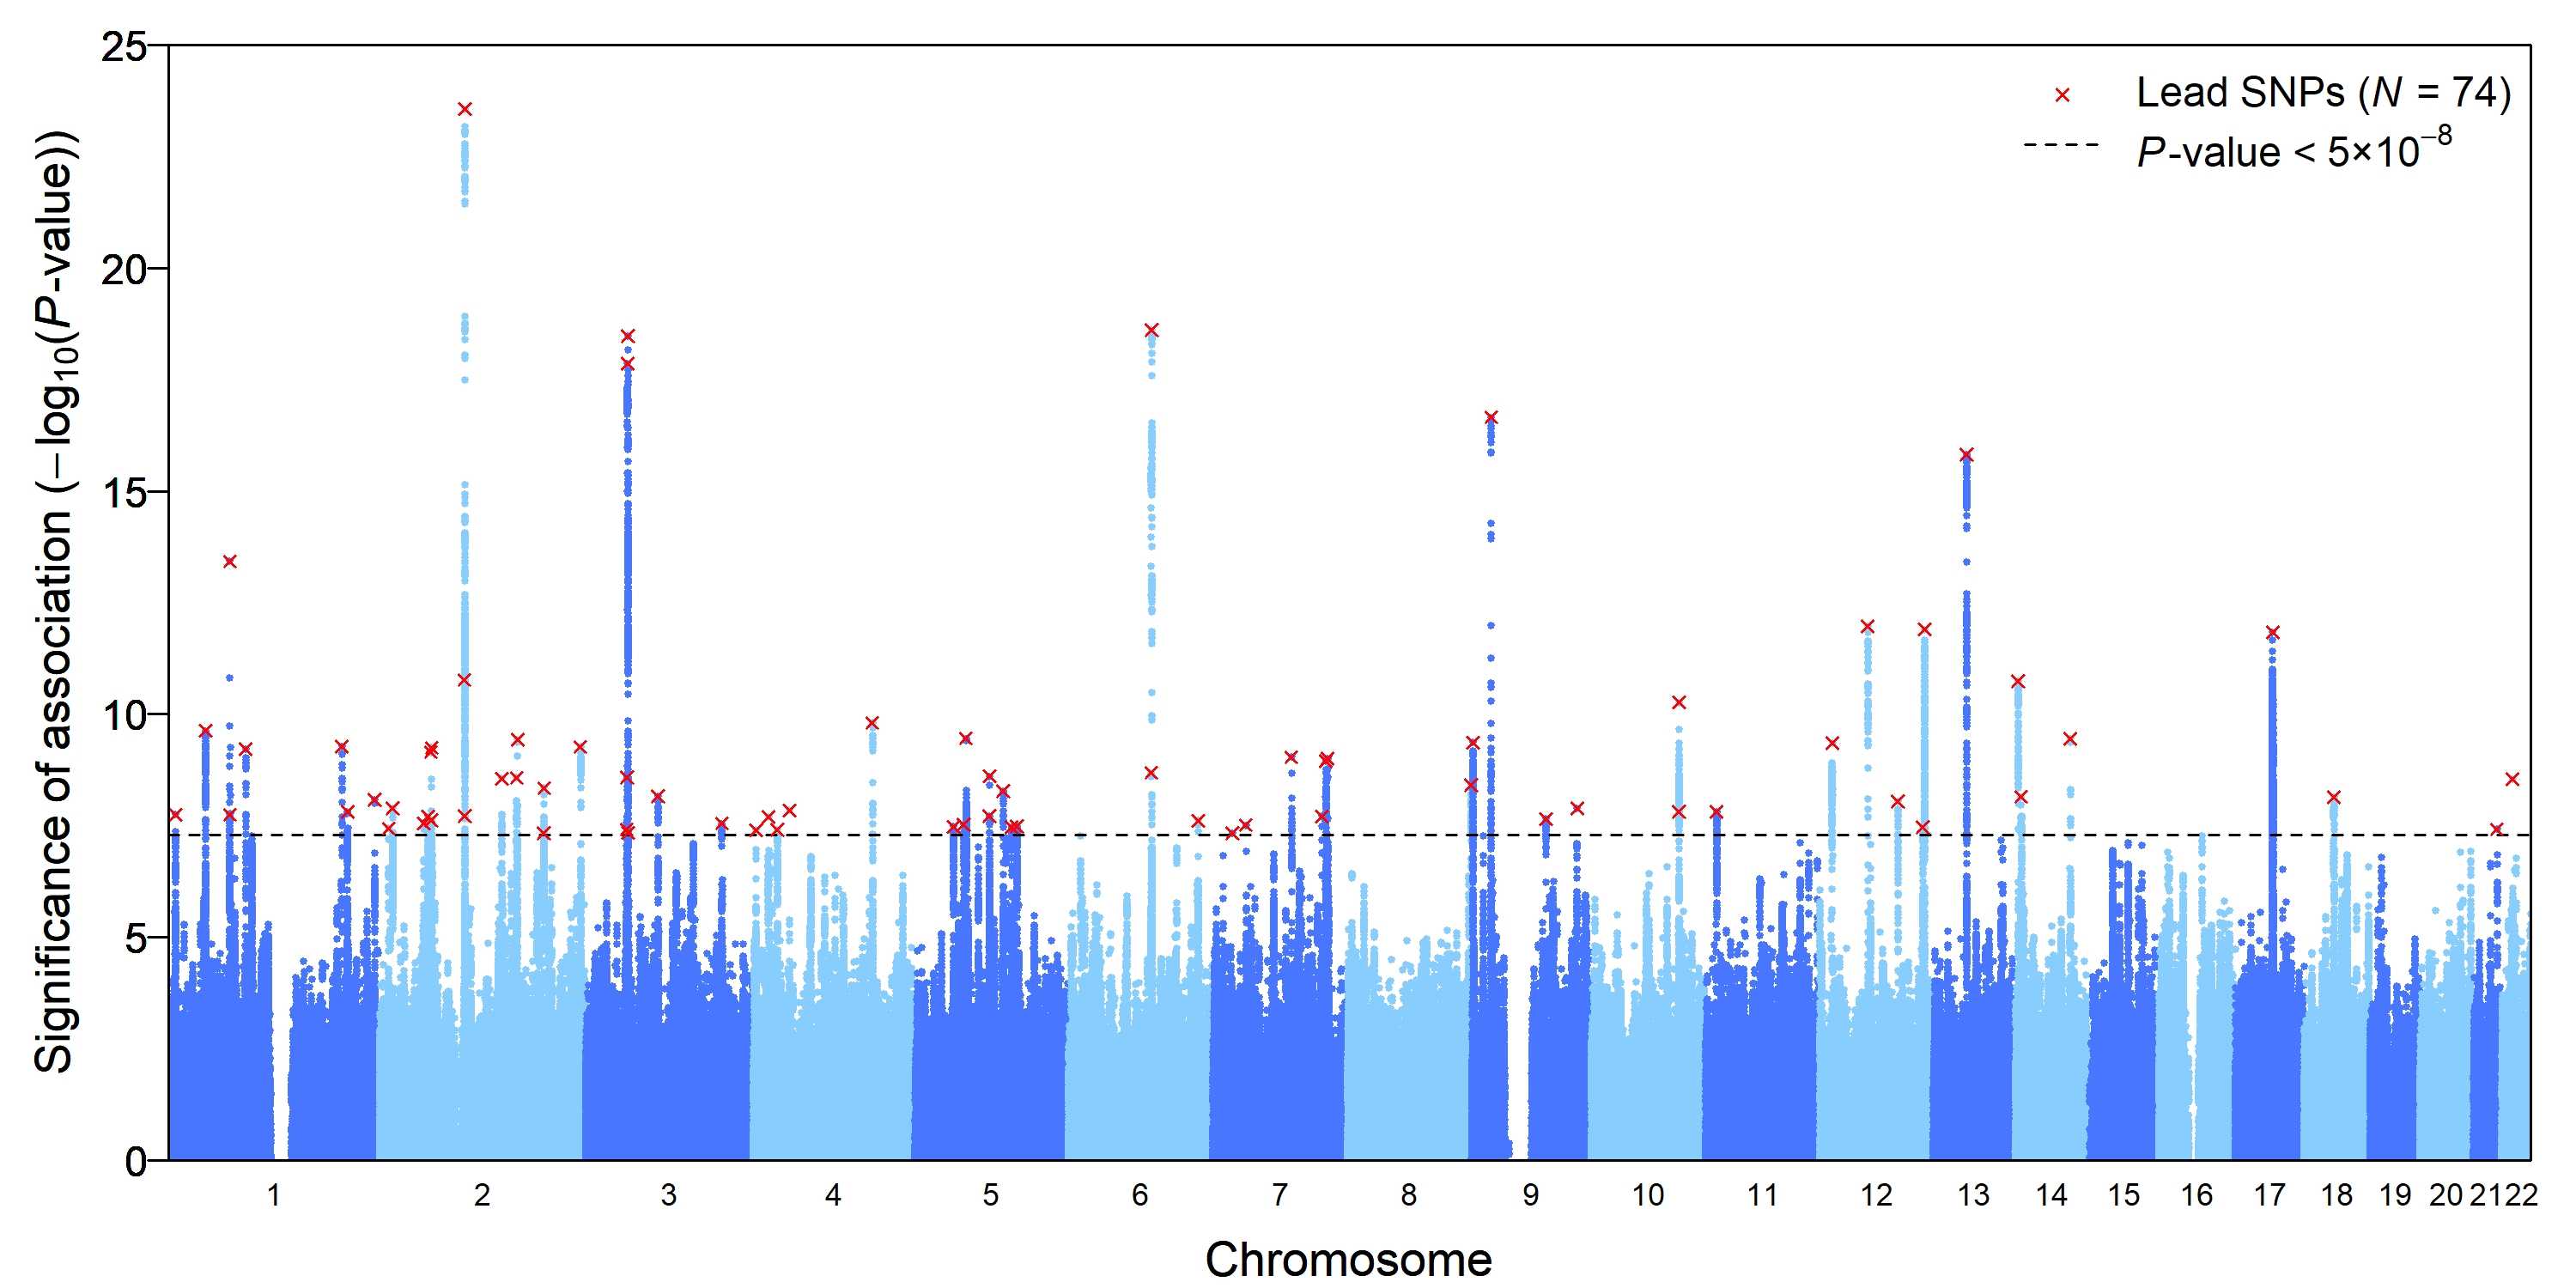
\includegraphics[width=14cm]{include/Manhattan_plot_EA2_EduYears_Pooled_Main_GxEpaper.jpg}
    \caption{Manhattan plot visualizing the results of the second genome-wide association study on educational attainment by \cite{okbay2016}.}
    \label{fig:manhattan}
\end{figure}

\subsection{Polygenic indices}
\label{sec:polygenicindices}
The tiny explanatory power of individual SNPs has led researchers to develop methods that combine individual SNPs into so-called polygenic indices (PGIs), which have substantially greater explanatory power. A PGI is a weighted sum of individual SNPs and reflects the best linear genetic predictor of the outcome \citep[e.g.,][]{Mills2020book,Becker2021}. It is constructed with the aim of predicting the genetic propensity toward a certain trait for individuals in a hold-out sample. For reasons of statistical independence, the hold-out sample cannot have been part of the original GWAS meta-analysis. 

In its most basic form, a PGI is constructed as follows: 
\begin{eqnarray}
PGI_i & = & \sum_{j=1}^{J} \beta_j^{GWAS} G_{ij},
\label{appeq:PGI}
\end{eqnarray}
where $G_{ij}$ is again the number of copies of the minor allele for individual $i$ and SNP $j$ and {\small $\beta_j^{GWAS}$} are the $\beta$ coefficients for SNP $j$ (see \autoref{eq:gwas2}) from the corresponding GWAS  \citep{dudbridge2013power}. By multiplying SNP $j$ (taking values $x_{ij} = \{0,1,2\}$) with its {\small $\beta_j^{GWAS}$} weight, SNPs with large effect sizes are weighted higher than those with small effect sizes. The simplest PGIs follow \autoref{appeq:PGI} where, given the linkage disequilibrium (LD) between SNPs, only one out of each genome-wide significant locus is maintained in the computation of the PGI.\footnote{More sophisticated construction measures exist that  leverage machine learning to account for LD \citep[see, for example,][]{so2017improving,Vilhjalmsson2015}, ancestry \citep{Marnetto2020}, or biological functioning \citep{liu2020leveraging,choi2023prset}, with typically better predictive power. However, all approaches have in common that they aggregate the genetic contributions of millions of small SNP-effects across the genome and are similar in spirit to the basic (and still used) approach of the linear weighted sum in \autoref{appeq:PGI}.}

PGIs that include all available SNPs (i.e., genome-wide significant as well as nonsignificant SNPs) typically explain most variation in the outcome \citep{Ware2017}. The predictive accuracy of a PGI is also an increasing function of the sample size of the GWAS \citep{dudbridge2013power}. As GWAS samples grow, the estimates of the $\beta_j^{GWAS}$ coefficients improve, and measurement error in the PGI is reduced. For example, whereas the PGI based on the first successful GWAS on educational attainment ($N \sim 125,000$) explained 3-4\% of the variance in educational attainment out-of-sample \citep{Rietveld2014}, the PGI based on the results of a second, third and fourth GWAS explained 6-8\%, 11-13\% and 13-16\% of the variation in educational attainment respectively \citep{okbay2016, lee2018gene, Okbay2022}. The maximum explained variance of a PGI is determined by the phenotype's so-called SNP-based heritability. Using methods like Genome-based Restricted Maximum Likelihood (GREML) estimation \citep{Yang2011}, several studies have shown that the SNP-based heritability of educational attainment is around 25\% in developed countries \citep{Rietveld2013}. In other words, today's PGI for educational attainment already explains a bit more than half the variation in educational attainment that is achievable.\footnote{Note that PGIs can also be used to explain variation in other traits than the trait on which it has been calibrated through the GWAS weight. For example, the EA PGI has been used to explain wealth \citep{papageorge2020genes} and health \citep{bolyard2024understanding} and in the present work we use it to explain test scores.} \cite{VanKippersluis2020} review and assess statistical approaches to correct the coefficient of the PGI for measurement error in a regression. These approaches are well-suited for purging measurement error in the main effect of the PGI in between-family settings, and relevant to use as long as the maximum explained variance of a PGI has not been reached. Because the PGI has no natural metric, its effects are typically reported in standard deviations on an underlying latent scale of (loosely speaking) genetic propensity \citep{Becker2021}.

\subsection{Epigenetics} \label{appsec:epi}
Here, we briefly discuss the relationship between $G \times E$ interplay and epigenetics. Genetic variants are fixed at conception and do not change over the lifetime. This makes them well-suited as right-hand side variables to study their effects on later-life outcomes, possibly in interaction with environments. In contrast, epigenetics is the study of the expression of genes, which by definition varies over time, and often also by tissue (e.g., expression in blood may be different from expression in skin tissue). This makes epigenetics more suited as a left-hand side variable (as done for instance in the epigenome-wide association study on educational attainment; \citet{karlsson2017epigenome}). If there is gene expression at a certain SNP, then epigenetics could be one mechanism through which $G \times E$ effects come into existence. However, there is no one-on-one translation from epigenetics to $G \times E$ interplay: 
    \begin{itemize}
    \item Epigenetics may also affect genetic variants that are not polymorphisms (i.e., that do not vary across humans). In contrast, $G \times E$ interactions can by definition only exist if there is variation in $G$ (SNPs);
    \item Even if a certain SNP exhibits expression, there could be compensatory investments that neutralize the initial $G \times E$ interaction;
    \item Even if a certain SNP does not exhibit gene-expression, there could still be $G \times E$ if certain `type' of individuals simply respond differently to a given environment.
    \end{itemize}
In sum, epigenetics is perfectly compatible with $G \times E$ and it is one of many potential mechanisms through which $G \times E$ may arise. However, it is neither a necessary nor sufficient condition for $G \times E$ (see \citet{baker2022beyond} for further discussion).  


\clearpage
\renewcommand{\thetable}{C.\arabic{table}}
\renewcommand{\thefigure}{C.\arabic{figure}}
\renewcommand{\theequation}{C.\arabic{equation}}
\setcounter{table}{0} 
\setcounter{figure}{0} 
\setcounter{equation}{0} 

\section{Discussion and illustrative derivations of biases} \label{appsec:bias}
The basic data generating process from \hyperref[subsec:ideal]{Section~\ref*{subsec:ideal}} is repeated here. The outcome $Y_i$ of child $i$ is a function of her genotype $G_i$, and the genotype of her mother $G_{m(i)}$ and of her father $G_{f(i)}$:
\begin{equation}
Y_i = \beta_0 + \beta_G G_i + \beta_{G_m} G_{m(i)} + \beta_{G_f} G_{f(i)} + \varepsilon_i,
\label{eq:Kong1app}
\end{equation}
where $\beta_0$ is a constant term, $\beta_G$ captures the direct genetic effect of the child's genotype $G_i$, and $\varepsilon_i$ denotes the error term. \citet{kong2020family} further specify the parameters $\beta_{G_m}$ and $\beta_{G_f}$ as $\beta_{G_m} = \eta_m +w$ and  $\beta_{G_f} = \eta_f +w$, where $\eta_m$ and $\eta_f$ denote genetic nurturing effects from the mother and father, respectively, and $w$ captures all confounding effects that have not been adjusted for, including assortative mating, sibling interactions, and contributions from older ancestors. 

Our ideal experiment discussed in \hyperref[subsec:ideal]{Section~\ref*{subsec:ideal}} includes parental genotypes $G_{m(i)}$ and $G_{f(i)}$ in both the GWAS as well as the $G \times E$ analysis stage. Assume for simplicity that $G_i$, $G_{m(i)}$ and $G_{f(i)}$ are all scalars with variance 1. Using a parent-child or sibling GWAS then will provide consistent estimates for $\beta_G$, $\beta_{G_m}$ and $\beta_{G_f}$. In turn, the true PGIs could be constructed as $PGI_i = \beta_G G_i$, $PGI_{m(i)} = \beta_{G_m} G_{m(i)}$, and $PGI_{f(i)} = \beta_{G_f} G_{f(i)}$. If in the analysis stage PGIs from both the child as well as both parents are included,
\begin{equation} 
    Y_i = \delta_0 + \delta_G PGI_{i} + \delta_{G_m} PGI_{m(i)} + \delta_{G_f} PGI_{f(i)} + e_i,
\end{equation}
then the $\delta$ parameters all provide unbiased estimates that converge to 1 asymptotically if the analysis sample has a perfect genetic correlation with the GWAS sample, the outcomes are identically measured, and the exact same SNPs are used in both the GWAS and construction of the PGIs. In the following subsections, we discuss various deviations from this ideal case. 



\subsection{Sibling effects} \label{appsec:siblingbias}


We first consider the case where there are two siblings and there is a direct effect $\beta_S$ of one's sibling's genotype on the other siblings' phenotype:
\begin{align} Y_{1j} &= \beta_{0j} + \beta_G G_{1j} + \beta_S G_{2j} + \varepsilon_{1j} \nonumber\\
 Y_{2j} &= \beta_{0j} + \beta_G G_{2j} + \beta_S G_{1j} + \varepsilon_{2j}. 
 \end{align}
In case we would be controlling for the parental genotypes $G_{m(i)}$ and $G_{f(i)}$, then both $\beta_G$ and $\beta_S$ would be estimated without bias, since offspring genotypes are random and conditionally independent. In a family fixed effects specification, however, this is not the case. 
When taking sibling differences to eliminate the family fixed effects, we obtain:
\[ Y_{1j}-Y_{2j} = \left(\beta_G - \beta_S\right) \left(G_{1j}-G_{2j} \right) + \left(\varepsilon_{1j}-\varepsilon_{2j}\right). \]
When $\beta_S$ is positive (negative), sibling effects cause a downward (upward) bias in the estimate of the effect of one's own genotype $G$, as measured by $\beta_G$.

\subsection{Interaction terms in family fixed effects models} \label{appsec:interactionfe}
Here, we consider the case with interaction terms in a family fixed effects model. If we add an interaction term to \autoref{eq:siblings}: 
\begin{align}
Y_{ij} &= \beta_{0j} + \beta_G G_{ij} + \beta_E E_{ij} + \beta_{G \times E} \left(G_{ij}\times E_{ij}\right) + \varepsilon_{ij} \nonumber\\
&= \beta_G \left(G_{ij}-\overline{G}_j\right) + \beta_E \left(E_{ij}-\overline{E}_j\right) + \beta_{G \times E} \left[ \left(G_{ij}\times E_{ij}\right)-\left(\overline{G_{ij}\times E_{ij}}\right)\right].
\label{eq:interactionfe}
\end{align}
The main effects of $G$ and $E$ are identified based on within-family variation, but the interaction term is not, since the deviation from the within-family product is not the same as the product of the within-family deviation. 

There is no perfect solution to this issue. Indeed, specifying an interaction between the family deviations $\left(G_{ij}-\bar{G}_j\right)$ and $\left(E_{ij}-\bar{E}_j\right)$ (rather than the deviation from the within-family product) is not a fixed effect specification as it would be a nonlinear transformation of the original interaction term since some observations would interact two negative values. It, therefore, generally does not generate meaningful estimates \citep{shaver2019interpreting}. So-called segmented (or stratified) regressions are sometimes performed \citep{shaver2019interpreting}, where one runs a within-family analysis to obtain the effect of $G$ stratified by different values of $E$, and vice versa. These analyses gauge whether the results are consistent with a positive or negative interaction. However, this solution is imperfect since stratification is based on potentially endogenous variables $G$ and $E$. An arguably more convincing approach would be to control for (imputed) parental genotypes directly in the specification with an interaction term. See, for instance, \cite{Muslimova2020b} for an empirical illustration and comparison of these different approaches.

\subsection{Not controlling for parental genotypes in GWAS and analysis stage} \label{appsec:underestimation}
In this subsection, we derive the consequences of not controlling for parental genotypes in the GWAS and/or analysis stage. Consider \autoref{eq:Kong1app} and assume random mating for simplicity. Under random mating, the correlation between the child's genotype $G_i$ and that of her parents is 0.5.\footnote{In practice, the correlation between siblings tends to be a little larger due to assortative mating. For example, \citet{torvik2022modeling} show how the raw correlation between sibling's EA PGI is around 0.55.} 

\paragraph{Parental genotypes in GWAS, but \textit{not} in analysis stage}
Let's first consider the case where one did include parental genotypes in the GWAS stage, but did not include parental PGIs in the analysis stage. In this case, we would estimate the true $PGI_i = \beta_G G_i$. In turn, since we do not include parental PGIs in the analysis stage:
\begin{align} 
 Y_i &= \delta_0 + \delta_G PGI_i + e \nonumber\\
  &= \delta_0 + \delta_G \beta_G G_i + e.
\end{align}
We can now derive that:
\begin{align}
 \hat{\delta}_G &= \frac{Cov(Y_i,\beta_G G_i)}{V(\beta_G G_i)} \nonumber\\
 &= \frac{Cov(\beta_0 + \beta_{G} G_i + \beta_{G_m} G_{m(i)} + \beta_{G_f} G_{f(i)} + \varepsilon_i,\beta_G G_i)}{V(\beta_G G_i)} \nonumber\\
 &= 1 + \frac{Cov(\beta_{G_m} G_{m(i)} + \beta_{G_f} G_{f(i)},\beta_G G_i)}{V(\beta_G G_i)} \nonumber\\
 &= 1 + \frac{0.5 \beta_{G_m} + 0.5 \beta_{G_f}}{\beta_G}.
\end{align}
Since $\beta_{G_m}$ and $\beta_{G_f}$ tend to have the same sign as $\beta_G$, coefficient $\delta_G$ would be overestimated because of the correlation between $PGI_i$ and the parental genotypes that are left out of the analysis stage. 

\paragraph{Parental genotypes not in GWAS, nor in analysis stage}
Now consider the common case where one did not control for parental genotypes in the GWAS stage, and also does not control for parental PGIs in the analysis stage. If we exclude parental genotypes from the GWAS stage, the child's estimated PGI is given by: 
\begin{equation} \label{eq:pginogwas}
    PGI_i = \left(\beta_G + 0.5 \beta_{G_m} + 0.5 \beta_{G_f} \right) G_i.
\end{equation}
In turn, since we do not include parental PGIs in the analysis stage:
\begin{align} \label{eq:notgwasnotanalysis}
 Y_i &= \delta_0 + \delta_G PGI_i + e \nonumber\\
  &= \delta_0 + \delta_G \left(\beta_G + 0.5 \beta_{G_m} + 0.5 \beta_{G_f} \right) G_i + e.
\end{align}
We can now derive that:
\begin{align}
 \hat{\delta}_G &= \frac{Cov(Y_i,\left(\beta_G + 0.5 \beta_{G_m} + 0.5 \beta_{G_f} \right) G_i)}{V(\left(\beta_G + 0.5 \beta_{G_m} + 0.5 \beta_{G_f} \right) G_i)} \nonumber\\
 &= \frac{Cov(\beta_0 + \beta_G G_i + \beta_{G_m} G_{m(i)} + \beta_{G_f} G_{f(i)} + \varepsilon_i,\left(\beta_G + 0.5 \beta_{G_m} + 0.5 \beta_{G_f} \right) G_i)}{\left(\beta_G + 0.5 \beta_{G_m} + 0.5 \beta_{G_f} \right)^2 V(G_i)} \nonumber\\
 &= \frac{\scriptstyle \beta_G^2 {+} 0.5 \beta_{G_m} \beta_G {+} 0.5 \beta_{G_f} \beta_G {+} 0.5\beta_{G_m} \beta_G {+} 0.25 \beta_{G_m}^2 {+} 0.25 \beta_{G_m} \beta_{G_f} {+} 0.5 \beta_{G_f} \beta_G {+} 0.25 \beta_{G_f} \beta_{G_m} {+} 0.25 \beta_{G_f}^2}{\left(\beta_G + 0.5 \beta_{G_m} + 0.5 \beta_{G_f} \right)^2} \nonumber\\
 &= 1.
\end{align}
Substituting $\delta_G=1$ back into \autoref{eq:notgwasnotanalysis} shows that the coefficient of $G_i$ does not just capture the direct genetic effect $\beta_G$, but instead also reflects the influence of parental genotypes and hence is overestimated whenever $\beta_{G_m}$ and $\beta_{G_f}$ are larger than zero. Thus, as this will typically be the case, not including parental PGIs in the analysis stage will lead to an upward bias in the coefficient of the direct genetic effect.

\paragraph{Parental genotypes not in GWAS, but only in analysis stage}
Finally, consider the case where one did not control for parental genotypes in the GWAS stage, but does include parental PGIs in the analysis stage. As before, if we exclude parental genotypes from the GWAS stage, the child's estimated PGI is given by equation \autoref{eq:pginogwas}, and the corresponding parental estimated PGIs are given by: 
\begin{equation}
PGI_{p} = \left(\beta_G +  0.5 \beta_{G_m} + 0.5 \beta_{G_f} \right) G_{p}. \qquad p=m,f
\end{equation}
In the analysis stage, we estimate:
\begin{align} Y_i &= \delta_0 + \delta_G PGI_i + \delta_{G_m} PGI_{m} + \delta_{G_f} PGI_{f} + e \nonumber\\
&= \delta_0 + \delta_G \left(\beta_G +  0.5 \beta_{G_m} + 0.5 \beta_{G_f} \right) G_i   + \delta_{G_m} \left(\beta_G +  0.5 \beta_{G_m} + 0.5 \beta_{G_f} \right) G_{m}  \nonumber\\
 & \qquad + \delta_{G_f} \left(\beta_G +  0.5 \beta_{G_m} + 0.5 \beta_{G_f} \right) G_{f} + e. \label{eq:tau}
 \end{align} 
Comparing \autoref{eq:tau} to the true data generating process from \autoref{eq:Kong1app}, it follows that:
\begin{equation}
    \delta_G \left(\beta_G +  0.5 \beta_{G_m} + 0.5 \beta_{G_f} \right) = \beta_G,
\end{equation} implying that 
\begin{equation} \label{eq:tauc_a}
\delta_G = \frac{\beta_G}{\left(\beta_G +  0.5 \beta_{G_m} + 0.5 \beta_{G_f} \right)}. 
\end{equation} Substituting $\delta_G$ from \autoref{eq:tauc_a} back into \autoref{eq:tau} shows that one can correctly recover the direct genetic effect $\delta$. Essentially, the coefficient of the misspecified PGI is scaled downwards (since $\delta_G < 1$ in \autoref{eq:tauc_a}) such that the estimated coefficient of the PGI only reflects the direct genetic effect. This is a special case however, one that corresponds to $\rho_g=1$ in \citet{Trejo2019}, where the correlation between the direct genetic effect and the genetic nurture effect is equal to 1. Intuitively, even though the GWAS coefficients used to construct the PGI are wrong, since the direct genetic effect $\beta_G$ and the genetic nurture effects $\beta_{G_m}$ and $\beta_{G_f}$ are proportional to each other (have correlation 1), including both the child's PGI and the parental PGIs enables to accurately scale these coefficients to retrieve the true direct genetic effects and genetic nurture effects. 

In general, this proportionality does not hold \citep{Trejo2019}. Consider again a highly stylized model to gain some intuition. We extend the model to two uncorrelated genetic variants $G_1$ and $G_2$, and to keep the notation tractable assume just one parent $p$ and ignore individual subscripts. Thus, the new data generating process is given by:
\begin{equation} \label{eq:dgp2}
 Y = \beta_0 + \beta_{G_1} G_1 + \beta_{G_2} G_2 + \beta_{G_{1p}} G_{1p} + \beta_{G_{2p}} G_{2p} + \varepsilon.
\end{equation}
If we exclude parental genotypes from the GWAS stage, the resulting PGI is estimated as
\begin{equation} \label{eq:pgi2}
 PGI = \left(\beta_{G_1} + 0.5 \beta_{G_{1p}} \right) G_1 + \left(\beta_{G_2} + 0.5 \beta_{G_{2p}}\right) G_2,
\end{equation}
and the parental $PGI_p$ is constructed analogously. If we now include the parental PGI as a control variable in the regression
\begin{align}
 Y &= \delta_0 + \delta_G PGI + \delta_{G_p} PGI_p + e \nonumber\\
 &= \delta_0 + \delta_G \Big[\left(\beta_{G_1} + 0.5 \beta_{G_{1p}} \right) G_1 + \left(\beta_{G_2} + 0.5 \beta_{G_{2p}}\right) G_2 \Big] \nonumber \\
 &\indent + \delta_{G_p} \Big[\left(\beta_{G_1} + 0.5 \beta_{G_{1p}} \right) G_{1p} + \left(\beta_{G_2} + 0.5 \beta_{G_{2p}}\right) G_{2p} \Big] + e.
\end{align}
To correctly retrieve the direct genetic effects $\beta_{G_1}$ and $\beta_{G_2}$, the following equalities should hold:
\begin{align}
\delta_G \left(\beta_{G_1} + 0.5 \beta_{G_{1p}}\right) & = \beta_{G_1}, \nonumber\\
\delta_G \left(\beta_{G_2} + 0.5 \beta_{G_{2p}}\right) &= \beta_{G_2}. 
\end{align}
Or, rearranged, 
\begin{align} \label{eq:tausimp}
\delta_G &= \frac{\beta_{G_1}}{\left(\beta_{G_1} + 0.5\beta_{G_{1p}}\right)} = \frac{1}{1 + 0.5 \frac{\beta_{G_{1p}}}{\beta_{G_1}}},  \nonumber\\
\delta_G &= \frac{\beta_{G_2}}{\left(\beta_{G_2} + 0.5 \beta_{G_{2p}}\right)} = \frac{1}{1+0.5 \frac{\beta_{G_{2p}}}{\beta_{G_2}}}.
\end{align}
Clearly, the two equalities of \autoref{eq:tausimp} are only satisfied if 
\begin{align}
\frac{\beta_{G_{1p}}}{\beta_{G_1}} = \frac{\beta_{G_{2p}}}{\beta_{G_2}}.
\end{align}
Thus, only when for all SNPs the genetic nurture effects are exactly proportional to the direct genetic effects (i.e., their correlation is 1), then it is possible to rescale the PGI coefficient to obtain the correct direct genetic effect using parameter $\delta_G$. In case the correlation between the direct genetic and genetic nurture effects is not perfect, there will be a downward bias in the estimated direct genetic effects. For a more general discussion, see \cite{Trejo2019}. 

\subsection{Endogeneity of \texorpdfstring{$E$}{}}
Endogeneity of $E$ may arise from five sources: reverse causality, omitted variable bias (especially from correlations with parental genotypes), measurement error, mediation, and correlation of the GWAS sample selection with the environment $E$. The last two sources of bias are discussed in the main text in \hyperref[subsec:endogenousE]{Section~\ref*{subsec:endogenousE}}. We discuss the other sources of bias here. We focus specifically on the resulting bias in the estimated coefficients of \autoref{eq:function} in a setting with gene--environment interplay. 

\paragraph{Bias arising from reverse causality:}
Especially in the case of a non-predetermined $E$, there may be reverse causality, with the outcome influencing the relevant environment. Such endogeneity will bias the estimated effect of $E$ and $G \times E$ but not the effect of $G$ if parental genotypes are used as controls. 

\paragraph{Bias arising from omitted environmental variables:}
Omitted variable bias can arise because environments typically do not arise in isolation. For instance, education, employment, and income are correlated with each other and with unobserved confounders. Therefore, even if a significant $E$ (or $G \times E$) is found, it is difficult to identify whether the association is driven by income, employment, education, or something else  \citep{Boardman2013}. Hence, endogeneity of $E$ implies that the coefficient on $G \times E$ may in fact reflect $G \times E^*$, i.e., a causal effect of some environment $E^*$ that is correlated with $E$. This is shown in the last two columns of \autoref{tab:Interpretation}. 

\paragraph{Bias arising from measurement error:}
A third source of endogeneity in $E$ is measurement error. If there is no $rGE$, then standard econometric theory explains how classical measurement error in $E$ will lead to attenuation bias. If there is no measurement error in $E$ but there is correlation between $G$ and $E$, the implications are more subtle: the known measurement error in PGIs as a proxy for $G$ will also lead to measurement error in $E$. Active $rGE$ implies that $G$ leads to self-selection into certain environments $E$. If in turn $G$ is measured with error, then not only is there attenuation bias in the coefficient of $G$, but also the coefficient of $E$ will be biased since the measurement error in $G$ introduces omitted variable bias in $E$.

\clearpage
\renewcommand{\thetable}{D.\arabic{table}}
\renewcommand{\thefigure}{D.\arabic{figure}}
\renewcommand{\theequation}{D.\arabic{equation}}
\setcounter{table}{0} 
\setcounter{figure}{0} 
\setcounter{equation}{0} 

\section{Representative examples from the literature} \label{sec:litreview}
We here discuss a representative study for each of the cells of  \autoref{tab:Interpretation}.\footnote{ \autoref{tab:Examples} in \autoref{appsec:MoreTabFig} includes the full list of studies on $G \times E$ interplay in human capital drawing on the EA PGI; for an extensive review of the cross-disciplinary literature on $G \times E$ interplay we refer to recent reviews \citep{domingue2020interactions,DiasPereira2022}.} 
A first observation from  \autoref{tab:Interpretation} is that there are currently no studies that exploit PGIs based on parent-child trio GWASs or within-family GWASs -- that is, there are no examples in the first row of the table. The first within-family GWASs \citep{Howe2022,Tan2024} were only recently published and to the best of our knowledge no studies exist that employed these summary statistics to construct a within-family PGI in a $G \times E$ analysis. Working from top-left to bottom-right, \citet{Muslimova2020b} is a study that uses a within-family design in the UK Biobank to study the interaction between the EA PGI and birth order to explain variation in educational attainment. Following the literature, they interpret birth order as a proxy for parental investments. The inclusion of family fixed effects renders the variation in PGIs across siblings random, and as an additional advantage one's birth order is also plausibly randomly assigned within-families. Indeed, the authors demonstrate that birth order and genetic variation are independent of one another, and that birth order-induced variation in educational attainment is thus environmental in origin. \citet{Muslimova2020b} show how both the EA PGI and birth order causally increase educational attainment. Furthermore, there is a non-negligible interaction between the two: firstborns with a polygenic index two standard deviations above the mean complete on average one extra year of education compared to their laterborn siblings with a similar polygenic index. Apparently, firstborn children benefit disproportionally from having a higher EA PGI, which is consistent with a the presence of a complementarity between endowments and investments in human capital production. 

\citet{houmark2022genetic} use the Danish iPSYCH data linked to administrative records on children's reading scores in elementary school to study the interaction between the EA PGI and an index of socioeconomic status (SES) of the family as measured by parental income and education. Their main results reflect between-family comparisons, but they also report findings from a smaller subsample of siblings. The findings from the within-family design are in the same direction, but they often lack statistical power since the sample size is substantially smaller, and the variation in the SES index is very limited across siblings. The authors show that both genetic as well as socioeconomic gaps in reading test scores between children increase throughout elementary school. Given their between-family design, they acknowledge that there exists some correlation across their SES measures and the PGI, but they also provide plausible evidence that the gaps largely open up independently. Their main finding is that the increase in the importance of the EA PGI with grade is completely driven by low SES children. This shows that a high EA PGI eventually leads to higher reading test scores among children from lower SES backgrounds. 

\citet{cheesman2022genes} draw on the Norwegian Mother, Father and Child Cohort (MoBa) data linked to Norwegian administrative records to study the interaction between the EA PGI and the social context as measured by schools and residential areas, on standardised national test results in maths, reading and English. In their analyses, they are able to control for parental EA PGIs ensuring that the variation in the child's EA PGI is exogenous. The authors use multilevel models where they allow for interactions between the EA PGI and random effects for the school and residential areas (neighborhood, district, and municipality). Their main finding is that the effect of the EA PGI is weaker in higher-performing schools: Differences between schools explain 4\% versus 2\% of the variance in educational achievement for children scoring 2 standard deviations below versus 2 standard deviations above the mean of the EA PGI. In contrast, there is no significant interaction between the EA PGI and residential environments. Whereas the study provides convincing evidence of $G \times E$ interactions in education, due to the endogeneity and latent measurement of school quality through random effects, they cannot identify the exact characteristic of the school that drives this pattern. 

Moving to the bottom row of \autoref{tab:Interpretation}, we have  \citet{Schmitz2017vietnam} being one of the earliest examples of a $G \times E$ analysis that exploits a plausibly exogenous $E$. The authors use the US Health and Retirement Study (HRS) to study the interaction between the EA PGI and Vietnam-era military service on educational attainment. In contrast to the UK Biobank, iPSYCH and MoBa datasets used in the studies reviewed above, the HRS does not include family-members (other than spouses). Therefore, the authors rely on a between-family design in which the EA PGI reflects both direct genetic effects as well indirect genetic effects. \citet{Schmitz2017vietnam} exploit an exogenous source of environmental exposure, the Vietnam-era draft lotteries, and thereby ensure that their $G$ and $E$ measures are not correlated to each other. Although their estimates do not reach statistical significance, possibly because of low statistical power, their findings suggest that draft eligible men with lower EA PGI scores completed fewer years of schooling. 

\citet{papageorge2020genes} also use HRS to study the interaction between various measures of parental SES and the EA PGI on educational attainment. The authors transparently show a modest association between the EA PGI and parental SES measures, including father's income and unemployment, and whether the family was financially well-off. \citet{papageorge2020genes} do control for parental education, which may go a long way in reducing concerns of $rGE$ and endogeneity of $G$. Their main finding is that the EA PGI has a negative interaction with parental SES in obtaining a high school degree, but a positive interaction in obtaining a college degree. Strengths of the relationships differ depending on the model specification. Interestingly, it seems that at lower levels of educational attainment, parental SES may substitute for genetic endowments, while parental SES could complement genetic endowments in college completion. 

Finally, \citet{arold2022genetic} use the U.S. National Longitudinal Study of Adolescent to Adult Health (AddHealth) to study the interaction between the EA PGI and school quality on educational attainment. They measure school quality as a composite measure (a principal component) capturing teacher experience, teacher turnover, teacher education, and class size. Whereas the authors adopt a between-family design in their main analysis and acknowledge that school quality may be endogenous, \citet{arold2022genetic} carefully address these concerns through a control function approach including rich measures of parental background and auxiliary analyses in a smaller sibling subsample. Their main finding is that the EA PGI and school quality are substitutes: a one-standard deviation increase in school quality reduces the effect of a one-standard deviation increase of the EA PGI by 20\%. Thus, high-quality teachers improve the chances of students with low genetic endowments to complete college.

These six representative studies draw on five datasets, from which the UK Biobank and the HRS are currently included in the polygenic index repository \citep{Becker2021}. Together, these six representative studies show that there is robust evidence of non-negligible $G \times E$ interactions in educational attainment. Returning to the motivations for studying $G \times E$ interplay from the introduction, even though all studies provide ex-post some theoretical grounding for the empirical findings, none of them offers a direct test of theoretically substantiated hypothesis. All six studies speculate about the mechanisms through which genetic factors operate, and some provide additional empirical analyses to substantiate such speculations \citep{Muslimova2020b,houmark2022genetic,papageorge2020genes,arold2022genetic}. Finally, all studies are informative about treatment effect heterogeneity, for some studies this analysis being the main motivation \citep{cheesman2022genes,Schmitz2017vietnam}.

Whereas we acknowledge that this is a selective set of studies that may be subject to publication bias, the estimates are also quantitatively meaningful. Where possible we benchmark the magnitude of the $G \times E$ coefficient to the main effect of $E$, i.e., the typical focus of studies in economics. In the preferred specification of \citet[][Table 2, last column]{Muslimova2020b}, the effect of birth order is 0.428 and the interaction term is estimated as 0.285, which constitutes 67\% of the main effect. It is worth noting that this is the only study in which measurement error in $G$ is addressed (using the approach developed by \cite{VanKippersluis2020}). In \citet[][Table B.2 in the Online Appendix]{papageorge2020genes}, the effect of father's income on college completion is estimated as 0.09 with an interaction term of 0.054 (i.e., 60\% of the main effect), and in \citet[][Table 3, column 1]{arold2022genetic} the effect of teacher quality is estimated to be 0.128 with an interaction term of -0.062 (i.e., 48\% of the main effect). At the lower end of the spectrum, \citet[][Table B1, column 3]{houmark2022genetic} estimate a coefficient of SES of 0.261 and an interaction term of 0.079, which represents roughly 30\% of the main effect. Finally, \citet[][Table 4, column 3]{Schmitz2017vietnam} the Vietnam draft has an estimated effect of -0.383 whereas the interaction term is non-significant and estimated to be -0.033 (i.e., 9\% of the main effect). Given the random slopes model, the presented estimates in \citet{cheesman2022genes} do not directly allow for a quantification of the interaction term with respect to the environmental main effect. Whereas the exact estimates vary depending on the environmental exposure, our selective set of studies shows that the interaction terms are typically a factor 1.5 to 3 smaller than the environmental main effect, but in virtually all cases meaningfully moderate the effect of the environmental exposure on educational attainment. 

\clearpage
\renewcommand{\thetable}{E.\arabic{table}}
\renewcommand{\thefigure}{E.\arabic{figure}}
\renewcommand{\theequation}{E.\arabic{equation}}
\setcounter{table}{0} 
\setcounter{figure}{0} 
\setcounter{equation}{0} 

\section{Steps in gene-environment interplay analysis} 
\subsection{Checklist} 
\label{sec:checklist}
Here, following the steps taken in the empirical application in the main text, we provide a simple checklist for applied researchers interested in estimating a form of gene--environment interplay. We assume that by the time the researcher is going through the checklist, she has already made a decision regarding the construction of the variables $Y$, $G$, and $E$:
\begin{enumerate}
    \item \textbf{Perform power calculations:}  
    Statistical power calculations have been a crucial element in genoeconomic analyses from the onset of the field \citep{Benjamin2011}. Since the anticipated effect sizes of interaction terms are typically an order of magnitude smaller than those of the main effects (see \autoref{sec:litreview}), it is strongly advised to conduct ex-ante power calculations before any empirical analysis is done. This avoids underpowered statistical tests and reduces the risk of finding false positives and negatives. Arguably the best way to mimic the actual statistical power of an empirical test for the interaction term is through simulations \citep{Duncan2011}. These allow one to specify the exact model that one intends to estimate and can account for possible adjustments to the standard error. In  \hyperref[powercalculationsapp]{Appendix~\ref*{powercalculationsapp}}, we provide the power calculations for our empirical application.
    
    \item \textbf{Check for gene--environment correlations $rGE$}:
    Check the extent to which genes correlate with the environment of interest (both endogenous and exogenous $E$ if possible). Finding no significant evidence for $rGE$ would help support the assumption that a truly exogenous environment is exploited in the analyses.
    \item \textbf{Investigate the correct functional form:} 
    Although $G \times E$ analyses are often conducted using linear interaction terms, it is advised to use descriptive analyses to check for nonlinearities in the relationship. To be as nonparametric as possible, one could plot the relationship between $G$ and $Y$ separately for the treated and control groups. Any difference in the $Y$-$G$ relationship between the treated and control groups is evidence in favor of $G \times E$. Differences in levels suggest that including $G$ and $E$ separately should suffice; differences in slopes between the two groups suggest a simple additive and linear specification with an interaction term; differences in only some parts of the distribution of the PGI suggest a more complex form of $G \times E$ interplay.\footnote{For a more thorough discussion of nonparametric analyses of gene--environment interplay in the context of a structural equation model (SEM), see \cite{Briley2015}. For more flexible functional forms additionally modeling possible heteroskedasticity, see \cite{Domingue2020.09.08.287888}.}
    \item \textbf{Perform $G \times E$ analysis:} 
    Perform the $G \times E$ analyses using the functional form determined in the previous step. Include all relevant control variables (e.g., principal components when within-family designs are not used). Interpret the findings in view of the mechanisms described in \hyperref[sec:econModel]{Section~\ref*{sec:econModel}} and assess the bias in the estimate based on \autoref{tab:Interpretation}. When exogeneity of $G$ or $E$ can only be guaranteed conditional on inclusion of certain control variables, one should always add interaction terms between each control variable and both the $G$ and $E$ terms. These additional interaction terms aim to capture any residual correlation between the controls and either genes or environment and are essential for estimating an unbiased effect of the interaction term \citep{Keller2014, feigenberg2023omitted}.
    \item \textbf{Correct inferences for heteroskedasticity and multiple hypothesis testing:} It is prudent to use robust standard errors in the analysis, and the analyst may wish to conduct heteroskedasticity tests as in \citet{Domingue2020.09.08.287888} if the variance of the outcome is expected to vary systematically with the environmental exposure. If the analysis involves many different outcomes explored under a more data-driven approach, one may want to correct for multiple hypothesis testing. 
\end{enumerate}


\subsection{Power calculations}
\label{powercalculationsapp}
We use simulations to perform \textit{ex-ante} power calculations to estimate the minimum detectable effect (MDE) for the $G \times E$ coefficient in our setting. Since the interaction term captures a form of nonlinearity in the relationship between $G$, $E$ and the outcome $Y$, simulations are arguably the most flexible and reliable way to approximate the actual statistical power of our empirical test \citep{Duncan2011}. We simulate the following (simplified) $G \times E$ model 1,000 times and approximate statistical power using the share of coefficients with a $p$ value $<0.05$:\footnote{The STATA code for these simulations and a simplified example code for simulating the statistical power of the empirical specification is available at our \href{http://github.com/geighei/GxE_4practitioners}{GitHub} or \href{https://zenodo.org/records/14968164}{Zenodo} repository. The example code allows one to specify a binary or continuous environment, different sample sizes, and other expected MDEs.}
%
\begin{equation} \label{eq:power}
    Y_i = \beta_0 + \beta_G G + \beta_E E + \beta_{G \times E} (G \times E) + \varepsilon.
\end{equation}
We set the parameters based on empirical results in the literature. Since our outcome variable $Y_i$ is always standardized to have mean 0 and standard deviation 1, we assume that $\alpha=0$ and that the error term is drawn from a standard normal distribution $\varepsilon \sim N(0,1)$. We also assume that $G$ is standard-normally distributed ($G \sim N(0,1)$), which is a good approximation of the distribution of the standardized PGI, and following \cite{Allegrini2019}, we set $\beta_G=0.259$.
Since approximately half of our sample is treated (i.e., born between September and November), we randomly assign 50\% of the simulated observations to have $E=1$ and the other half $E=0$. Following \cite{Crawford2010}, we assume that $\beta_E=0.90, 0.60, 0.35, 0.20$ and $0.13$ when the outcome is the Entry Assessment) score, KS1, KS2, KS3, and KS4, respectively.\footnote{Note that \cite{Crawford2010} do not report estimates for the Entry Assessment test. We hypothesize this to be $0.90$, in line with the pattern of greater effect sizes for younger children. Indeed, as we show below, our results for the Key Stages are remarkably similar to these authors' estimates: 0.70 (KS1), 0.39 (KS2), 0.22 (KS3) and 0.28 (KS4), as shown in \autoref{tab:MoB_ks}.} Finally, given our ALSPAC data, we set the sample size in the power calculations to $N=1,000$ for the Entry Assessment score, $N=3,500$ for Key Stages 1, 2 and 4, and $N=3,000$ for Key Stage 3.

\autoref{fig:power} shows the statistical power that we can expect for each outcome variable and for different magnitudes of the interaction coefficient $\beta_{G \times E}$ from \autoref{eq:power}. Following the literature,\footnote{See our discussion of the size of $G \times E$ estimates in the existing literature at the end of \autoref{sec:litreview}. Regarding treatment effect heterogeneity in school starting age effects, \cite{Crawford2010} do not report this based on either individual or parental characteristics. However, \cite{Black2011} report heterogeneity of effects based on a composite measure of parental background (see Table 7 in their paper). Moving from the bottom 25\% to the top 75\% of the distribution (a shift equivalent to about 2 standard deviations in our PGI distribution), the effect of early age-at-entry more than doubles for outcomes such as education, earnings at age 35, and teenage pregnancy but does not differ for outcomes such as IQ or mental health. We take a conservative approach and consider a change of about one-quarter of the main effect of the environment.} % 
we expect the magnitude of the interaction effect to be about one-quarter of the size of the main effect of the environment. Therefore, we expect $\beta_{G \times E}=0.225, 0.15, 0.0875, 0.05$ and $0.0325$ when the outcome is the Entry Assessment score, KS1, KS2, KS3, and KS4, respectively. Hence, we have more than 90\% power to estimate the interaction effect for the Entry Assessment score and about 75\% power for KS1, although we are underpowered for the other outcomes.
More generally, we are well powered ($>80\%$) to estimate an interaction coefficient greater than 0.1 for the Key Stage outcomes and greater than 0.175 for the Entry Assessment test. 

\begin{figure}[H]
\centering 
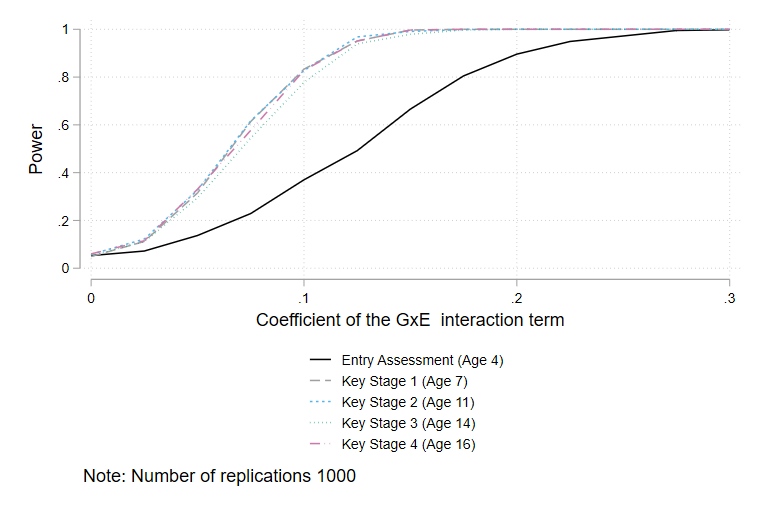
\includegraphics[width=0.7\linewidth]{include/power.png}
\caption{Power calculations for detecting the interaction coefficients in \autoref{tab:MoB_ks}.}
\label{fig:power}
\end{figure}

\clearpage
\renewcommand{\thetable}{F.\arabic{table}}
\renewcommand{\thefigure}{F.\arabic{figure}}
\renewcommand{\theequation}{F.\arabic{equation}}
\setcounter{table}{0} 
\setcounter{figure}{0} 
\setcounter{equation}{0} 

\section{Robustness analyses} \label{appsec:robustness}

\subsection{Non-linearities in \texorpdfstring{$G$}{G}}
In this Appendix, we explore the robustness of our estimates. First, although \autoref{fig:PGIxTreat_ea} suggests that we can approximate the relationship between the PGI and the outcome as linear, we explore the robustness of our results to non-linearities in the PGI effect, following \hyperref[sec:econModel]{Section~\ref*{sec:econModel}}.

\autoref{tab:MoB_G2} shows that the coefficient on PGI$^2$ is insignificantly different from zero in most specifications; the exception being for the KS3 (age 13-14) outcome. This again suggests that a linear relationship between the PGI and the outcome fits the data well. The addition of the square of the child's PGI also does not lead to large differences in the estimates of the control variables. Comparing \autoref{tab:MoB_G2} to the same specification (but without quadratics) in \autoref{tab:MoB_ea} and \autoref{tab:MoB_ks} shows that the parameter of interest ($\delta_{G \times E}$) is generally robust to the inclusion of the quadratic term, though the addition of the parental PGIs increases the standard error somewhat, reducing the precision of the estimate. 

\addtolength{\tabcolsep}{-0.35em}
\renewcommand{\arraystretch}{0.75}
\begin{table}[h]
\caption{OLS estimates of the main and interaction effects of being old-for-grade (Treated) and the EA
PGI on children’s test scores, allowing for non-linearities (quadratic) in the PGI effect.}
\centering
{\scriptsize
\begin{tabular}{lcccccccccccccccccccc}
\toprule
\input include/MoB_G2b
\bottomrule
\addlinespace[.75ex]
\end{tabular}
\label{tab:MoB_G2}
}
\caption*{\scriptsize \noindent \textit{Notes:} The analysis uses a bandwidth of 3 months before and after the September cutoff (i.e., June till November). Additional control variables include gender, year of birth, the first 10 principal components, a dummy for missing parental PGI, and interactions of all covariates with PGI Child and with Treated. Robust standard errors in parentheses, clustered by month of birth. * $p < 0.10$, ** $p < 0.05$, *** $p < 0.01$.}
\end{table}

\subsection{Bandwidth}
In our main specification we set the bandwidth to three months before and after September to balance bias and precision. This choice, however, remains somewhat arbitrary. Here we investigate the robustness of our results against using smaller or larger bandwidths. \autoref{tab:MoB_bandwidth} shows the results specifying different bandwidth for the RDD, including two and four months on either side of the threshold. Our main results are robust to the use of different bandwidths, with the estimate of interest generally being somewhat larger in the analysis with a two-month bandwidth, and smaller in the analysis with a four-months bandwidth. Despite the bigger sample size in the latter, the standard errors are consistently larger, and the estimates are not significantly different from zero.

\addtolength{\tabcolsep}{-0.15em}
\begin{table}[h]
\caption{OLS estimates of the main and interaction effects of being old-for-grade (Treated) and the EA
PGI on children’s test scores, exploring sensitivity to different bandwidths.}
\centering
{\scriptsize
\begin{tabular}{lcccccccccccccccccccc}
\toprule
\input include/MoB_bandwidth
\bottomrule
\addlinespace[.75ex]
\end{tabular}
\label{tab:MoB_bandwidth}
}
\caption*{\scriptsize \noindent \textit{Notes:} The analysis uses a bandwidth of two or four months before and after the September cutoff. Additional control variables include gender, year of birth, the first 10 principal components, a dummy for missing parental PGI, and interactions of all covariates with PGI Child and with Treated. Robust standard errors in parentheses, clustered by month of birth. * $p < 0.10$, ** $p < 0.05$, *** $p < 0.01$.}
\end{table}


\clearpage
\begin{landscape}
\section{Additional Figures and Tables} 
\renewcommand{\thetable}{G.\arabic{table}}
\renewcommand{\thefigure}{G.\arabic{figure}}
\renewcommand{\theequation}{G.\arabic{equation}}
\setcounter{table}{0} 
\setcounter{figure}{0} 
\setcounter{equation}{0} 
\label{appsec:MoreTabFig}

\begin{table}[H] \caption{Empirical examples of $G \times E$ studies using the EA PGI in gene--environment interaction models.} \label{tab:Examples}
\centering
{\scriptsize
\begin{tabular}{llll} 
\hline \hline \\
& \multicolumn{1}{c}{Exogenous $E$} & \multicolumn{2}{c}{Endogenous $E$} \\ 
\cmidrule(lr){2-2}\cmidrule(lr){3-4} \\
& \multicolumn{1}{c}{} & \multicolumn{1}{c}{Predetermined $E$} & \multicolumn{1}{c}{Non-predetermined $E$} \\ 
\\
\hline
& & & \\

Exogenous $G$ (parent-child/sibling) \&       &  &  \\
\indent\hspace{0.3cm} PGI on basis of parent--child GWAS       &         &  & \\
 &   &   &  \\

\hline
&&&\\

Exogenous $G$ (parent-child/sibling) \&        & \citet[][Birth order]{Muslimova2020b} & \citet[][Family circumstances]{Bates2018} & \citet[][Social context]{cheesman2022genes} \\
\indent\hspace{0.3cm} PGI on basis of regular GWAS  &  \citet[][Education system]{Barcellos2021}  & \citet[][Family circumstances]{Domingue2015a}  &  \\
& \citet[][Vaccination campaign]{berg2023early} &  \citet[][Family circumstances]{houmark2022genetic}&\\
& & \citet[][Family circumstances]{ronda2022family} &\\
& & \citet[][Cohort/Family circumstances]{pettersson2023genetic} &\\
&&& \\
\hline
& & & \\

Endogenous $G$ (between family data) &  \citet[][Education system]{ahlskog2024testing} & \citet[][Adoption status]{cheesman2020comparison} & \citet[][Various, some predetermined]{allegrini2020multivariable}\\
\indent\hspace{0.3cm} PGI on basis of regular GWAS &  \citet[][Pollution reduction programme]{fukushima2024long} & \citet[][Family circumstances]{conley2015effect} & \citet[][Teacher quality]{arold2022genetic}\\
 & \citet[][Education system]{Johnson_demography} &  \citet[][Cohort]{conley2016changing} & \citet[][Various]{nagpal2022canalization}\\    
 & \citet[][Collapse political system]{Rimfeld2018} & \citet[][Birth weight]{conley2019birth} &  \citet[][Mental health]{rajagopal2020polygenic} \\
 & \citet[][Vietnam draft]{Schmitz2017vietnam} &   \citet[][Cohort]{Pereira2021.12.14.472565}  & \\ 
 & \citet[][Collapse political system]{ujmaeducational}  & \citet[][Socioeconomic context]{fletcher2019decoupling} &  \\
& \citet[][Prenatal sugar consumption]{berg2023prenatal}   &  \citet[][Family circumstances]{isungset2022social} &  \\
& \citet[][London smog]{von2022long}  & \citet[][Family circumstances/Cohort]{lin2020social} & \\
  && \citet[][Socioeconomic context]{mills2018gene}  &\\
  && \citet[][Cohort]{muslimova2022rank}  &\\
  && \citet[][Cohort]{okbay2016}  &\\

&  & \citet[][Family circumstances]{papageorge2020genes} & \\
&   & \citet[][Family circumstances]{Selzam2016} & \\
&   & \citet[][Family circumstances]{von2020predicting} & \\
&   & \citet[][Family/School circumstances]{uchikoshi2021gene} & \\
&  & \citet[][Family circumstances]{wickrama2021early}& \\
\\
\hline \hline
\end{tabular}}
\caption*{\footnotesize {\textit{Notes:} $G$ stands for genotype, $E$ for environment, $E^*$ for environments \textit{other than} those of interest, and $rGE$ for gene--environment correlation. A predetermined environment $E$ is defined as an environment not causally influenced by one's genes $G$ yet possibly correlated with other environmental characteristics $E^*$ and potentially shaped by parental genes.}}
\end{table}
\end{landscape}

\renewcommand{\thetable}{G.\arabic{table}}
\renewcommand{\thefigure}{G.\arabic{figure}}
\renewcommand{\theequation}{G.\arabic{equation}}
\setcounter{table}{1} 
\setcounter{figure}{0} 
\setcounter{equation}{0} 

\begin{figure}[H]
\centering 
\caption{Densities of children's, mothers' and fathers' EA PGI by treatment status.}
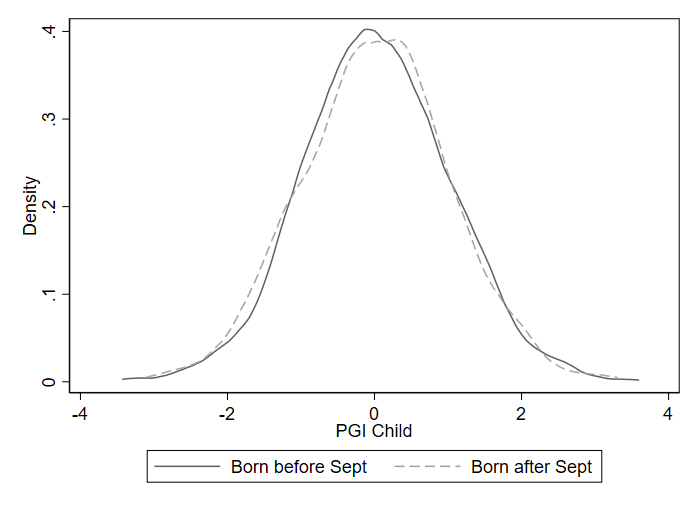
\includegraphics[width=0.49\linewidth]{include/kdens_treat_PGS.png} \\
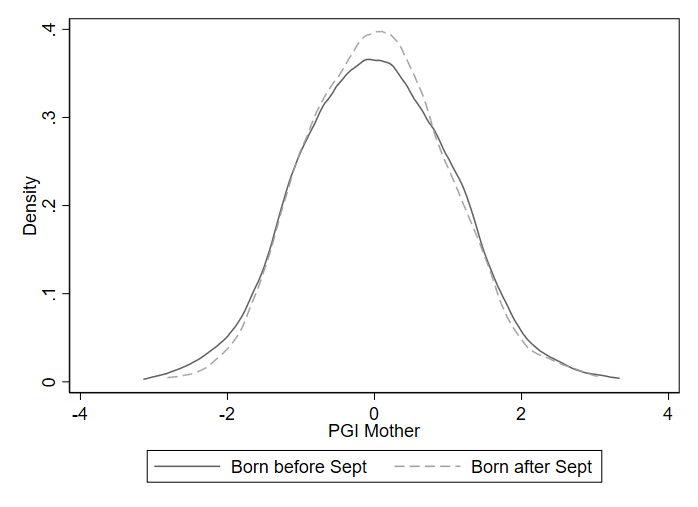
\includegraphics[width=0.49\linewidth]{include/kdens_treat_PGS_mothers.png}
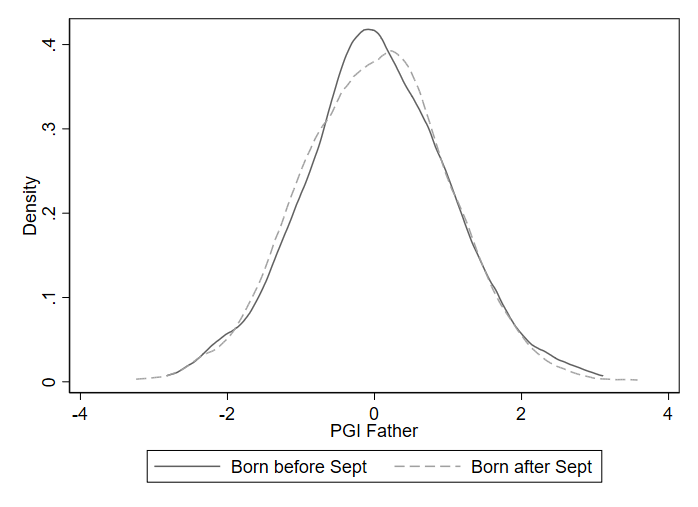
\includegraphics[width=0.49\linewidth]{include/kdens_treat_PGS_fathers.png}
\label{fig:kdens_treat_PGI}
\end{figure}

\begin{figure}[ht]
\centering 
\caption{The $G \times E$ coefficients for the Entry Assessment and Key Stage 1--4 test scores.}
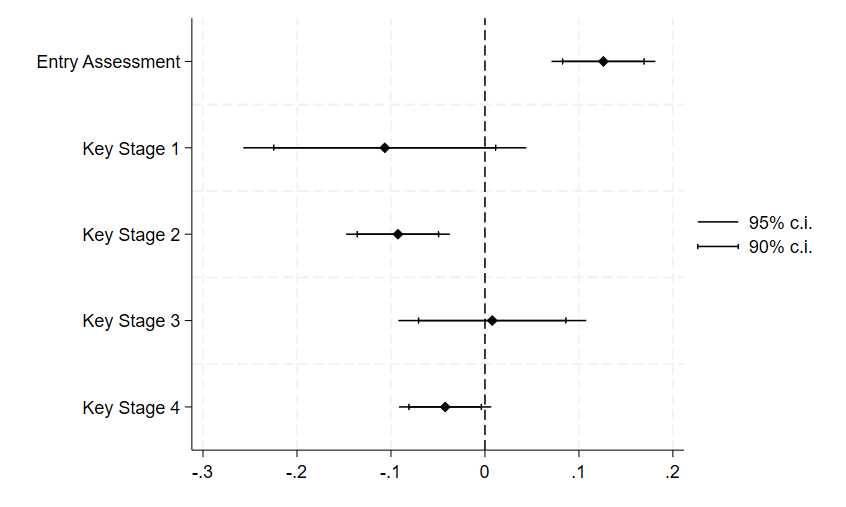
\includegraphics[width=0.6\linewidth]{include/coefplot_gxe.png}
\label{fig:coefplot}
\end{figure}

\addtolength{\tabcolsep}{0.3em}
\begin{table}[H]
\caption{OLS estimates of the effect of the parental PGIs for EA on test scores at different ages.}
\centering
{\footnotesize
\begin{tabular}{lcccccccccccccccccccc}
\toprule
\input include/PredictivePower_23me_ukb_app
\bottomrule
\addlinespace[.75ex]
\end{tabular}
\label{tab:PredictivePowerApp}
}
\caption*{\footnotesize \noindent \textit{Notes:} The test score and the EA PGI are standardized to have mean 0 and standard deviation 1 in the analysis sample. All regressions control for gender and the first ten principal components of the genetic data, as well as a dummy if the parental PGIs are missing. Robust standard errors in parentheses. * $p < 0.10$, ** $p < 0.05$, *** $p < 0.01$.}
\end{table}

\clearpage 
\begin{spacing}{1.0}
\setlength{\bibsep}{0.0pt}
\renewcommand\refname{References (Appendix)}
\putbib[genes]
\end{spacing}
\end{bibunit}

\end{document}